\documentclass[UTF8,fontset=windows,zihao=-4,a4paper]{ctexart}

% 页面与字体：正文小四宋体、单倍行距、无页眉、页脚居中页码
\usepackage{geometry}
\geometry{top=2.35cm,bottom=2.35cm,left=2.45cm,right=2.45cm}
\usepackage{amsmath,amssymb}
\usepackage{graphicx}
\usepackage{booktabs}
\usepackage{tabularx}
\usepackage{makecell}
\usepackage{array}
\usepackage{multirow}
\usepackage{float}
\usepackage{caption}
\usepackage[numbers,sort&compress]{natbib}
\usepackage{xcolor}
\usepackage{enumitem}
\usepackage[hidelinks]{hyperref}

\graphicspath{{figs/}}
\captionsetup{font=small,labelfont=bf,labelsep=quad,justification=centering}
\ctexset{
  section/name={第,章},
  section/format={\centering\heiti\zihao{4}},
  section/beforeskip={1.0ex plus 0.3ex minus 0.2ex},
  section/afterskip={0.8ex plus 0.2ex},
  subsection/format={\heiti\zihao{-4}},
  subsubsection/format={\heiti\zihao{-4}}
}
\setlength{\parindent}{2em}
\setlength{\parskip}{0.15em}
\setlength{\emergencystretch}{3em}
\linespread{1.02}
\setlist{nosep,leftmargin=2em}
\renewcommand{\arraystretch}{1.12}

\begin{document}
\pagenumbering{arabic}
\pagestyle{plain}

\begin{center}
{\heiti\zihao{3} 基于随机森林与共表达网络融合的啤酒风味预测}\\[0.25em]
{\heiti\zihao{3} 及关键化合物识别}
\end{center}

\vspace{0.6em}

\section{摘要}

啤酒风味是数百种化合物在酿造与陈酿过程中共同作用的结果，具有维度高、样本少、共线性强的特点。本文以 \textbf{250} 个啤酒样本的 \textbf{231} 个化学特征和 \textbf{50} 个感官维度为对象，建立“数据口径统一—\textbf{随机森林}回归—分级标定—\textbf{共表达网络}融合排序”的建模框架，并对模型进行多角度检验。

\textbf{针对问题一}，将感官评分预测写成 \textbf{50} 维多输出回归，采用 \textbf{随机森林}（由多棵决策树平均的集成模型）拟合化合物与感官维度之间的非线性关系，再用\textbf{锚定线性映射与四舍五入}（ALR）把连续预测转成 \textbf{0--6} 级整数。两阶段预注册选型得到随机森林与 \textbf{226} 维特征集 F0，折外 \textbf{R\textsuperscript{2}} 为 \textbf{0.2565}、五折均值为 \textbf{0.2305}，高于同口径基线 \textbf{0.243}。针对 \textbf{0} 级与 \textbf{6} 级为空的现象，本文证明这是\textbf{刻度不可达命题}：折外预测为条件均值，预测与标签的标准差之比为 \textbf{0.444}，方差比约 \textbf{0.197}，与 \textbf{R\textsuperscript{2}} 同阶；锚点冻结时 \textbf{6} 级要求预测越过标签约 \textbf{92} 百分位，故两端等级不可达是口径的数学必然，而非实现缺陷。辅助的\textbf{可读口径}表在保持单调同序（逆序对 \textbf{0}）的前提下使 \textbf{7} 级全部出现。

\textbf{针对问题二}，以 \textbf{226} 个候选化合物为节点、以 \textbf{Spearman} 秩相关绝对值不低于 \textbf{0.30} 为边，构建含 \textbf{3758} 条边的共表达网络；将直接相关得分与邻居加权得分按 \textbf{0.70} 的图项权重融合，为每个感官维度给出 \textbf{Top-3} 关键化合物。\textbf{Bootstrap} 重采样 \textbf{200} 次显示，第一名化合物的平均入选频率为 \textbf{0.6734}，第三名降至 \textbf{0.3611}；\textbf{Jaccard} 重合度为 \textbf{0.378}，说明图项确实改变了排序。以来源品类核对，一致 \textbf{48} 对、不一致 \textbf{86} 对、不可比 \textbf{16} 对，一致率 \textbf{0.3582}，高于独立基线 \textbf{0.2047}。\textbf{梯度提升机}（GBM）全局对照中 \textbf{60/60} 的重合由候选池包含关系恒真，本文只把平均分位 \textbf{0.6201} 对 \textbf{0.4971} 作为有信息量的证据。

\textbf{针对问题三}，题面要求以风格为条件生成化合物谱与感官画像并做跨风格迁移。本文只给出条件生成、化学约束与回评的拟采用路线，不报告任何结果，具体见第 \textbf{6} 章。

最后，本文用缺失扰动、锚点扰动和外部证据检验模型：缺失比例增至 \textbf{20\%} 时折均 \textbf{R\textsuperscript{2}} 由 \textbf{0.2305} 降至 \textbf{0.2121}，分级一致率仍为 \textbf{0.8882}；外部证据 E1、E2、E3 的方向一致率分别为 \textbf{0.9968}、\textbf{0.8098}、\textbf{0.9706}。模型在可解释性与稳健性之间取得了可复核的平衡。

\noindent\textbf{关键词：}啤酒风味预测；随机森林；共表达网络；分级标定；稳定性分析；关键化合物识别；小样本高维建模

\section{问题重述与分析}

\subsection{问题背景}

啤酒的香气与风味由醇、酯、酸、硫化物、萜烯等多类化合物共同决定。同一化合物在不同浓度区间可能呈现水果香、花香、麦芽香或异味，不同化合物之间还存在加成、掩盖与协同作用。仅凭单一化合物的浓度很难解释整体感官印象，因此需要把化学测量、感官评分与化合物之间的关联结构放在同一个框架中分析\cite{jiang2018}。本题给出 \textbf{250} 个啤酒样本的化学特征、\textbf{50} 个感官维度、化合物相关矩阵以及若干辅助属性表，要求依次完成感官评分预测、关键化合物识别和风格条件生成三项任务。数据驱动的建模方法为这类高维小样本问题提供了可行路径\cite{zhang2020}。

\subsection{问题一的重述与分析}

\textbf{重述：}问题一要求根据每个啤酒样本的化学特征，预测其在 \textbf{50} 个感官维度上的 \textbf{0--6} 级评分。训练数据包含 \textbf{231} 个化学特征和 \textbf{50} 个连续感官标签，标签需要按题面评分卡转成整数等级；评价时既关心连续预测的拟合程度，也关心分级结果是否保持原有顺序与分布形态。

\textbf{分析：}这一问的本质是“高维输入、小样本、多输出”的回归问题。难点有三：其一，\textbf{231} 个特征之间存在明显共线性，线性模型容易过拟合；其二，样本只有 \textbf{250} 个，而每个感官维度都要单独建模，折外预测的方差会被放大；其三，题面要求输出 \textbf{0--6} 的整数，而连续预测的分布通常比标签更集中，直接四舍五入会丢失两端等级。针对这些难点，本文用随机森林捕捉非线性与交互作用\cite{breiman2001}，用固定折索引的交叉验证控制评估偏差\cite{li2019}，再把连续预测送入预先冻结的 ALR 标定规则；对两端等级为空的现象，不通过拉伸预测去“补”，而是给出可检验的机理解释与可读口径辅助表。

\subsection{问题二的重述与分析}

\textbf{重述：}问题二要求利用化合物相关矩阵建立共表达网络，并结合化学特征与感官标签，为每个感官维度找出 \textbf{3} 个关键化合物；同时要说明结果的稳定性、化学合理性，并与全局重要度排序进行对照。

\textbf{分析：}这一问的核心不是“算一个相关系数”，而是“在相关结构上做可解释的排序”。直接按化合物与感官维度的相关系数排序，容易选中彼此高度共线的“同伙”，忽略与目标化合物协同起作用的邻居；只按网络中心性排序，又会脱离感官目标。因此本文采用“直接相关得分 + 邻居加权得分”的融合分数，把图结构作为平滑项而不是替代项。稳定性用有放回重采样衡量，化学合理性用化合物来源品类与感官维度的对应关系核对，全局对照只作为旁证，避免把恒真的集合包含关系误读为重要度一致。多重比较用 Benjamini--Hochberg 方法控制错误发现率\cite{benjamini1995}。

\subsection{问题三的重述与分析}

\textbf{重述：}问题三要求以啤酒风格为条件，学习一个能够生成化合物谱与对应感官画像的模型，并考察生成结果在不同风格之间的迁移能力。题面同时要求生成结果在化学上可解释、在感官上可核对。

\textbf{分析：}这一问与问题一、问题二的方向相反：前两问是“由化合物到感官”的判别与排序，这一问是“由风格到化合物谱”的条件生成。难点在于风格标签的样本量不均衡、化合物维度高且存在大量零值与强相关，生成器很容易只记住训练风格而失去迁移能力。本文拟采用“风格条件编码—化合物谱生成—感官回评—化学约束”的路线，把问题一的预测器作为回评器，把问题二的关键化合物作为化学约束的落点；本阶段只登记路线与验证设计，不报告任何生成结果。

\subsection{总体思路}

全文按“先统一口径、再分别建模、最后交叉检验”的顺序展开。第 \textbf{3} 章登记数据口径与预处理；第 \textbf{4} 章解决问题一，重点是随机森林回归、ALR 标定和刻度不可达命题；第 \textbf{5} 章解决问题二，重点是共表达图、融合排序、稳定性与化学合理性；第 \textbf{6} 章给出问题三的题面要求与拟采用路线；第 \textbf{7} 章评价模型并给出结论与建议。三问共用同一套样本口径与特征命名，避免在不同章节出现互相矛盾的数字。

\section{数据与预处理}

\subsection{数据构成与统一口径}

本题的数据分为化学测量、感官评分、化合物相关结构、外部证据和辅助说明五类。本文先按文件登记用途与规模，再统一样本键、特征名和维度顺序；后续各章只引用本表登记的口径，不在正文中另立一套数字。数据文件与用途如表 \ref{tab:data-files} 所示。

\begin{table}[H]
\centering
\zihao{5}
\begin{tabularx}{\textwidth}{@{}p{0.14\textwidth}p{0.15\textwidth}X p{0.28\textwidth}@{}}
\toprule
数据块 & 规模 & 主要内容 & 本文用途与处理 \\
\midrule
\texttt{1.csv} & \textbf{250}$\times$\textbf{234} & 样本标识、\textbf{231} 个化学特征 & 问题一输入；问题二计算逐维直接相关时按列内可用样本成对计算 \\
\texttt{2.csv} & \textbf{231}$\times$\textbf{231} & 化合物之间的 Spearman 相关矩阵 & 问题二建图；剔除 \textbf{4} 个聚合列与热量列后保留 \textbf{226} 个候选节点 \\
\texttt{3.xlsx} & 评分卡 & \textbf{0--6} 七档人工评分与公式 & 只用于核对分级语义与维度映射，不直接取数 \\
\texttt{4.csv} & \textbf{250}$\times$\textbf{50} & \textbf{50} 个感官维度的连续标签 & 问题一目标；问题二逐维直接相关的另一侧 \\
\texttt{5.csv} & \textbf{50}$\times$\textbf{50} & 感官维度之间的相关阵 & 独立证据 E2 的参照 \\
\texttt{6.csv} & \textbf{44}$\times$\textbf{50} & 化学指标与感官维度的参考相关 & 独立证据 E1 的参照；\textbf{42} 个指标可映射到 \texttt{1.csv} \\
\texttt{7.csv} & \textbf{186} 个属性 & 细粒度风味属性与三个视角 & 独立证据 E3 的参照；\textbf{39} 个属性可桥接 \\
\texttt{8.xlsx} & 多工作表 & 阈值、可读名、来源品类、GBM 全局重要度 & 名称对齐、化学合理性核对与全局对照 \\
\bottomrule
\end{tabularx}
\caption{数据文件、规模与本文用途}
\label{tab:data-files}
\end{table}

表 \ref{tab:data-files} 中 \texttt{5.csv}、\texttt{6.csv} 与 \texttt{7.csv} 只作为独立证据，不参与问题一的训练，也不参与问题二的 Top-3 计算。这样安排的目的，是让“用来拟合的数据”和“用来核对的数据”保持分离，避免把同一份信息既当输入又当验证。

\subsection{与题面口径的差异登记}

题面对样本数、感官维度数和辅助表规模使用的是近似口径，与仓库内数据文件逐格核对后存在差异。按照“以数据文件为准、差异只登记不反过来改数据”的原则，本文统一采用表 \ref{tab:caliber} 的实测口径；题面数字只在表 \ref{tab:caliber} 中出现一次，后续正文不再使用。

\begin{table}[H]
\centering
\zihao{5}
\begin{tabularx}{\textwidth}{@{}p{0.18\textwidth}p{0.16\textwidth}p{0.16\textwidth}X@{}}
\toprule
项目 & 题面写法 & 实测口径 & 差异说明与处理 \\
\midrule
样本数 & \textbf{226} & \textbf{250} & \texttt{1.csv} 与 \texttt{4.csv} 均有 \textbf{250} 行，按 \texttt{beer} 键 250/250 对齐；以 \textbf{250} 为准 \\
感官维度 & 约 \textbf{40} 维 & \textbf{50} 维 & \texttt{4.csv} 剔除 \texttt{beer}、\texttt{beer\_id}、\texttt{tasting\_category\_fine} 后为 \textbf{50} 列 \\
化学特征 & 约 \textbf{226} 种 & \textbf{231} 个特征 & \textbf{231} = \textbf{226} 个单一化合物 + \textbf{4} 个聚合列 + \textbf{1} 个热量列 \\
外部指标 & \textbf{46} 项 & \textbf{44} 项 & \texttt{6.csv} 实有 \textbf{44} 行；其中 \textbf{42} 项可映射到 \texttt{1.csv} \\
细粒度属性 & \textbf{187} 项 & \textbf{186} 项 & \texttt{7.csv} 实有 \textbf{186} 个属性；其中 \textbf{39} 个可桥接到感官维度 \\
\bottomrule
\end{tabularx}
\caption{题面口径与实测口径的差异登记}
\label{tab:caliber}
\end{table}

除表 \ref{tab:caliber} 的规模差异外，源表还有三类需要注意的细节。第一，\texttt{4.csv} 与 \texttt{summary} 在三个维度名上存在拼写差异，例如 \texttt{A\_esters\_fruity} 与 \texttt{A\_ester\_fruity}，本文以 \texttt{4.csv} 为准。第二，\texttt{summary} 的 C 组列序与 \texttt{4.csv} 不同，任何按位置取列的做法都会错位，必须先按名称建索引。第三，\texttt{summary} 中 \texttt{barnyard} 与 \texttt{stale\_hops} 指向同一单元格，属于源表公式缺陷；本文直接使用 \texttt{4.csv} 的两列独立数据，缺陷只登记、不修复源文件。

\subsection{缺失、变换与名称对齐}

\texttt{1.csv} 的 \textbf{231} 个特征共有 \textbf{73} 个缺失格，占 \textbf{250}$\times$\textbf{231} 个格子的 \textbf{0.126\%}，分布在 \textbf{9} 列；缺失最多的是 \texttt{amyl.acetate}，有 \textbf{27} 格，其次是 \texttt{aroma\_hops\_sum} 的 \textbf{13} 格和 \texttt{methylpyrazine} 的 \textbf{12} 格。问题二建图使用 \texttt{2.csv} 的相关系数矩阵，不依赖逐样本完整行，因此不插补；问题一在训练折内按风格分组取中位数，组内样本少于 \textbf{5} 个时回退到全局中位数，并为 \textbf{9} 个有缺失的列各保留一列缺失标记，避免把“补过的值”和“原始值”混在一起。

特征变换按列判定。对 \texttt{1.csv} 与校准表可比的 \textbf{70} 列逐列比较 \texttt{log10} 与自然对数，\textbf{70/70} 列都是 \texttt{log10} 的绝对误差更小，其中 \textbf{37} 列在 \texttt{log10} 下精确成立；另有 \textbf{33} 列本来就是原始量纲，不做反变换。这个判定直接影响问题三的浓度域，也影响问题一对 \textbf{33} 个原始量纲列的预处理：这 \textbf{33} 列在建模前做 \texttt{log10}$(x+10^{-6})$，其余 \textbf{198} 列保持原值。

名称对齐是问题二的前置条件。\texttt{2.csv} 的节点名与 \texttt{1.csv} 的字段名并不完全一致，本文先做大小写、希腊字母和非字母数字的归一化，再用 \texttt{8.xlsx} 的 \texttt{field\_name\_R} 到 \texttt{chemical\_name} 的桥接表补齐，最终 \textbf{231/231} 个特征全部找到唯一节点，且没有重复目标。三处命名怪例（\texttt{dihydroiso}\allowbreak\texttt{caryophyllene.epoxide} 对 \texttt{Tobacarol}、\texttt{selin.11.en.4.alpha.ol} 对 \texttt{Kongol}、\texttt{X2.ethylhexylsalicylate} 对 \texttt{2-ethylhexyl acrylate}）按源表原样保留，不做人工改写。

\subsection{预处理流程与防泄漏}

问题一的预处理固定为六步，顺序不可交换。第一步按 \texttt{beer} 整数键对齐 \texttt{1.csv} 与 \texttt{4.csv}，250/250 全部命中；不使用 \texttt{beer\_id}，因为它在两张表中的精度不同。第二步对 \textbf{33} 个原始量纲列做 \texttt{log10}$(x+10^{-6})$。第三步在训练折内做分组中位数插补，并保留缺失标记。第四步在训练折内做 z-score 标准化，测试折只用训练折的均值和标准差。第五步保留 \texttt{4.csv} 的连续标签原值，不再做变换，以免破坏 ALR 锚点的语义。第六步保留全部 \textbf{250} 行样本，不删除异常样本。

防泄漏的关键在第三、四步：插补参数和标准化参数都只从训练折估计，测试折不参与。折划分使用固定的五折索引，每折 \textbf{50} 个样本，所有模型、所有特征集、所有感官维度共用同一组折，保证不同方案之间的差异只来自模型或特征集，而不是折的随机性。问题二不训练预测器，只对 \texttt{1.csv} 与 \texttt{4.csv} 做成对秩相关，因此其缺失处理与问题一不同：不插补、不删行，按列内可用样本计算并在结果中保留样本量。

\subsection{数据质量对建模的影响}

数据质量对三问的影响并不相同。对问题一，\textbf{73} 个缺失格只占 \textbf{0.126\%}，但集中在少数列，若直接删行会损失样本，若用全表中位数又会把测试折信息带进训练，因此采用训练折内分组中位数加缺失标记。对问题二，\texttt{2.csv} 是题方给出的相关矩阵，不能按 \texttt{1.csv} 的缺失重新计算，否则会改变图结构；本文只把它当作固定的图输入，另用 \texttt{1.csv} 成对计算逐维直接相关。对问题三，\textbf{33} 个原始量纲列与 \textbf{37} 个对数可精确反解列的区分，决定了浓度域是否差一个数量级，必须在生成模型之前固定，不能等到生成后再补救。

\section{问题一：感官评分的多输出回归与分级}

\subsection{问题描述}

问题一给出 \textbf{250} 个啤酒样本的 \textbf{231} 个化学特征，要求预测每个样本在 \textbf{50} 个感官维度上的评分，并把连续预测转成题面规定的 \textbf{0--6} 级整数。记化学特征矩阵为 $X\in\mathbb{R}^{250\times 231}$，感官标签矩阵为 $Y\in\mathbb{R}^{250\times 50}$，第 $d$ 个感官维度的标签为 $y_d$。学习目标是构造映射 $f_d\colon\mathbb{R}^{231}\to\mathbb{R}$，使折外预测 $\hat y_d=f_d(X)$ 与 $y_d$ 的误差尽可能小；随后用固定规则把 $\hat y_d$ 转成整数等级 $s_d\in\{0,1,\ldots,6\}$。

这一问的困难不在单个回归器的实现，而在三组矛盾。第一，特征多、样本少：\textbf{231} 个特征对应 \textbf{250} 个样本，若用线性模型，共线性会把系数估计放大；第二，多输出之间并不独立：麦芽香、酒花香、酯香等维度在感官上相关，逐维建模会重复利用同一批信息；第三，连续预测与离散评分之间存在“刻度差”：题面要的是 \textbf{0--6} 的等级，而模型输出的是条件均值，二者的分布形态并不相同。本文的模型设计分别回应这三组矛盾。

\subsection{模型建立}

\subsubsection{多输出随机森林}

本文把 \textbf{50} 个感官维度视为 \textbf{50} 个独立的回归任务，共用一个随机森林结构。随机森林由 $T$ 棵回归树组成，第 $t$ 棵树在自助采样得到的训练子集上生长，叶节点取该节点样本标签的均值。对输入 $x$，森林预测为
\begin{equation}
\hat y_d(x)=\frac{1}{T}\sum_{t=1}^{T}\hat y_{d,t}(x),
\label{eq:rf}
\end{equation}
其中 $\hat y_{d,t}(x)$ 是第 $t$ 棵树对第 $d$ 维的输出。树的每次分裂选择使左右子节点平方误差之和下降最多的特征与切分点，即
\begin{equation}
\Delta \mathrm{SSE}= \mathrm{SSE}(S)-\mathrm{SSE}(S_L)-\mathrm{SSE}(S_R),
\label{eq:split}
\end{equation}
其中 $S$ 为当前节点样本集，$S_L$、$S_R$ 为切分后的左右子集。随机森林在每次分裂时只随机考虑一部分特征，并对样本做有放回采样，因而能降低单棵树的方差，适合本题这种特征相关、样本有限的场景\cite{zhou2016,breiman2001}。

本文不把 \textbf{50} 个维度合并成一个多任务模型，而是逐维独立训练。这样做的好处是每一维的损失只由该维标签决定，不会因为某些维度量纲不同而互相牵制；代价是计算量随维度线性增加。考虑到 \textbf{50} 维、\textbf{250} 样本的规模，这一代价可以接受。

\subsubsection{ALR 分级标定}

连续预测 $\hat y_d$ 不能直接四舍五入成 \textbf{0--6}：不同维度的标签取值范围不同，直接取整会把大量样本压到 \textbf{0} 或 \textbf{1}。本文采用分维锚定线性映射加四舍五入（Anchor--Linear--Round，ALR）。对第 $d$ 维，取标签的 \textbf{0.5\%} 与 \textbf{99.5\%} 分位数为锚点 $lo_d$、$hi_d$，先做线性映射
\begin{equation}
s_d^{\ast}=6\cdot\frac{\hat y_d-lo_d}{hi_d-lo_d},
\label{eq:alr-linear}
\end{equation}
再按“半数向上”取整并截断：
\begin{equation}
s_d=\min\left\{6,\max\left\{0,\left\lfloor s_d^{\ast}+0.5\right\rfloor\right\}\right\}.
\label{eq:alr-round}
\end{equation}
式 \eqref{eq:alr-linear} 把不同量纲的预测拉到同一把 \textbf{0--6} 尺子上，式 \eqref{eq:alr-round} 保证输出是整数且不越界。锚点只从标签分布估计，不从预测分布估计；这一点是后文“刻度不可达命题”的前提，也是本文不通过拉伸预测去填补空等级的原因。

\subsubsection{评价指标}

连续预测用决定系数和平均绝对误差评价：
\begin{equation}
R^2=1-\frac{\sum_{i=1}^{n}(y_i-\hat y_i)^2}{\sum_{i=1}^{n}(y_i-\bar y)^2},\qquad
\mathrm{MAE}=\frac{1}{n}\sum_{i=1}^{n}\left|y_i-\hat y_i\right|.
\label{eq:metrics}
\end{equation}
$R^2$ 越接近 \textbf{1} 表示拟合越好，负值表示不如直接用均值预测；MAE 越小表示平均绝对偏差越小。分级结果另用单调性、保序性、等级覆盖、往返一致性和信息损失等指标检验，具体判据在第 \ref{sec:q1-check} 节给出。

\subsection{算法求解}

\subsubsection{预处理与验证设计}

预处理严格按第 \textbf{3} 章登记的口径执行：按 \texttt{beer} 键对齐 \textbf{250} 个样本；对 \textbf{33} 个原始量纲列做 \texttt{log10}$(x+10^{-6})$；在训练折内按风格分组取中位数插补 \textbf{73} 个缺失格，并保留 \textbf{9} 个缺失标记列；在训练折内做 z-score 标准化；\textbf{50} 维标签保持原值；全部 \textbf{250} 行参与建模。

交叉验证采用固定五折，每折 \textbf{50} 个样本，随机种子为 \textbf{2026}。所有模型、所有特征集、所有维度共用同一组折索引，折外预测由五折测试段拼接而成。这样得到的 OOF 预测既用于连续指标，也用于 ALR 分级；全量重训模型的样本内预测只用于推理接口自测，不进入任何论文数值。

随机森林的超参数在建模前冻结：树数 \textbf{500}，最大深度 \textbf{8}，叶节点最少样本 \textbf{3}，每次分裂随机考虑 \textbf{33\%} 的特征，随机种子 \textbf{2026}。本文不做网格搜索，也不逐维调参，避免在 \textbf{50} 维上产生选择偏差。

\subsubsection{两阶段模型选择}

模型选择分两阶段预注册，第二阶段只看一个指标。第一阶段固定 \textbf{230} 维特征集 F1，比较岭回归、随机森林和直方图梯度提升机；岭回归只作线性对照，不参与选型。第二阶段用胜出的随机森林分别跑 \textbf{226} 维的 F0、\textbf{230} 维的 F1 和 \textbf{231} 维的 F2，按“提升不足 \textbf{0.02} 就不加特征”的三步决策表判定。这个阈值在跑结果之前写入方案，结果出来之后不回改。

三步决策的逻辑是：若 F2 相对 F1 的提升达到 \textbf{0.02}，采用 F2；否则若 F1 相对 F0 的提升达到 \textbf{0.02}，采用 F1；否则采用最简的 F0。该规则把“特征更多是否真的有用”变成一个可复算的阈值判断，而不是凭测试集表现挑一套特征。

\subsubsection{求解流程}

求解按以下顺序执行：读取 \texttt{1.csv} 与 \texttt{4.csv} 并按 \texttt{beer} 对齐；按第 \textbf{3} 章的六步预处理生成训练折与测试折；在 F1 上训练三个候选模型并记录五折平均 $R^2$；用胜出的随机森林在 F0、F1、F2 上重复同一组折；按决策表选出主模型与主特征集；用五折 OOF 预测做 ALR 标定，得到 \textbf{250}$\times$\textbf{50} 的评分表；最后计算 T1--T8、E1--E3 与缺失鲁棒性指标。整条流程只依赖固定折索引与固定随机种子，冷跑与复跑应逐格一致。

\subsection{求解结果}

\subsubsection{模型与特征集}

模型选择结果如表 \ref{tab:q1-select} 所示。第一阶段中，随机森林的五折平均 $R^2$ 为 \textbf{0.2304}，明显高于直方图梯度提升机的 \textbf{0.1343}；岭回归为 \textbf{-0.6585}，说明线性模型在 \textbf{231} 维共线特征上严重过拟合。第二阶段中，F0、F1、F2 的平均 $R^2$ 分别为 \textbf{0.2305}、\textbf{0.2304}、\textbf{0.2317}，F1 相对 F0 的变化为 \textbf{-0.000095}，远小于 \textbf{0.02} 的阈值，因此决策表命中步骤 \textbf{3}，采用 F0。

\begin{table}[H]
\centering
\zihao{5}
\begin{tabularx}{\textwidth}{@{}p{0.10\textwidth}p{0.18\textwidth}rrrrX@{}}
\toprule
阶段 & 方案 & 特征数 & 折均 $R^2$ & OOF 全局 $R^2$ & 折均 MAE & 判定 \\
\midrule
阶段一 & 岭回归（对照） & \textbf{230} & \textbf{-0.6585} & \textbf{-0.4977} & \textbf{0.5039} & 不参与选型 \\
阶段一 & 随机森林 & \textbf{230} & \textbf{0.2304} & \textbf{0.2579} & \textbf{0.3390} & 主模型 \\
阶段一 & 直方图梯度提升机 & \textbf{230} & \textbf{0.1343} & \textbf{0.1850} & \textbf{0.3524} & 候选 \\
阶段二 & 随机森林 $\times$ F0 & \textbf{226} & \textbf{0.2305} & \textbf{0.2565} & \textbf{0.3394} & 采用 \\
阶段二 & 随机森林 $\times$ F1 & \textbf{230} & \textbf{0.2304} & \textbf{0.2579} & \textbf{0.3390} & 否 \\
阶段二 & 随机森林 $\times$ F2 & \textbf{231} & \textbf{0.2317} & \textbf{0.2583} & \textbf{0.3387} & 否 \\
\bottomrule
\end{tabularx}
\caption{问题一的模型选型与特征集决策}
\label{tab:q1-select}
\end{table}

表 \ref{tab:q1-select} 中“折均 $R^2$”是五个测试折上 \textbf{50} 维平均 $R^2$ 的再平均，“OOF 全局 $R^2$”是把五折测试段拼成 \textbf{250} 行后一次性计算的全局值，两者不可混比。主模型在 OOF 全局口径下为 \textbf{0.2565}，高于同口径的基线 \textbf{0.243}；在同折基线口径下，折均 \textbf{0.2305} 也高于 \textbf{0.2122}。两种口径下都不低于基线，说明增益不是换口径造成的。

\begin{figure}[H]
\centering
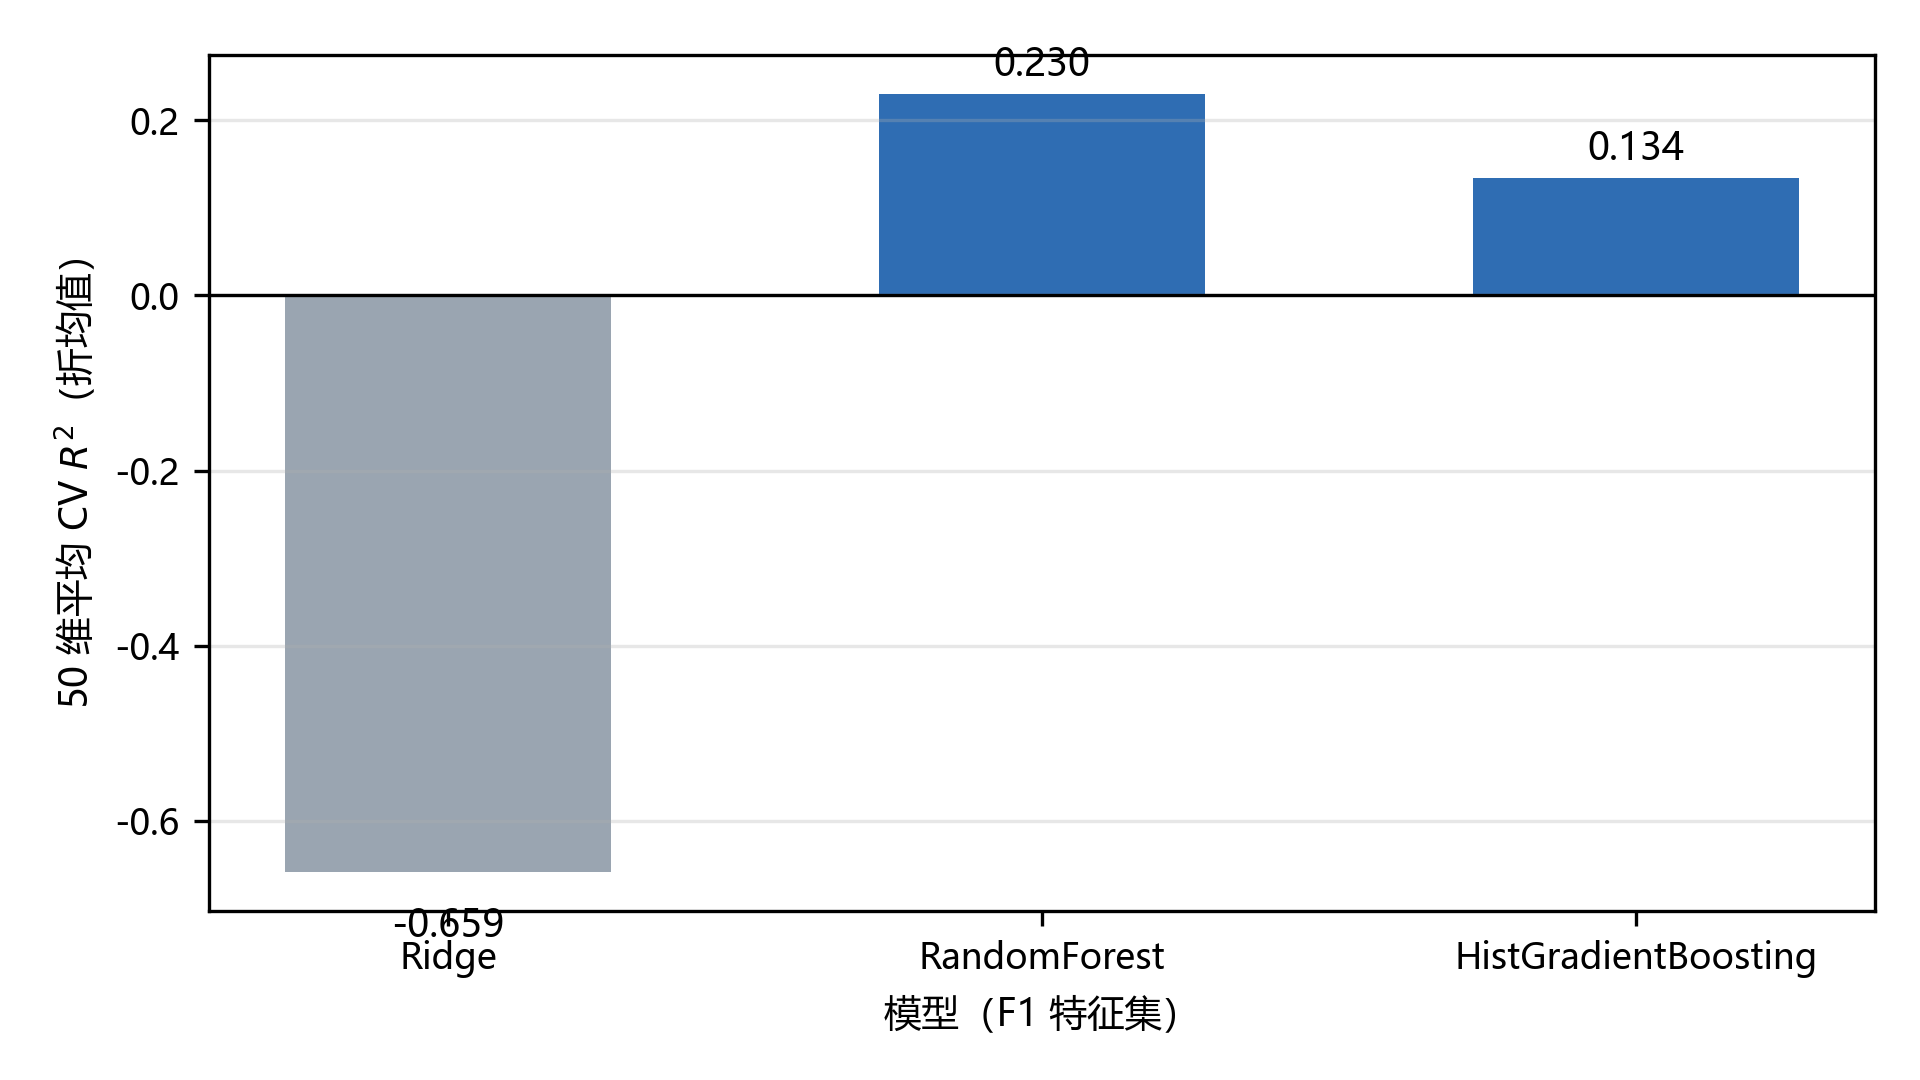
\includegraphics[width=0.68\textwidth]{图M3-01-模型选型对比.png}
\caption{三个候选模型在 F1 特征集上的 \textbf{50} 维平均交叉验证 $R^2$}
\label{fig:q1-model}
\end{figure}

图 \ref{fig:q1-model} 把三种模型的差距压缩成一张条形图：随机森林的柱高明显高于梯度提升机，岭回归则落到零线以下。需要说明的是，岭回归的负值不是“模型坏了”，而是线性假设与本题的强非线性、强共线性不匹配；它的作用只是提供一个“线性不可用”的对照。

\begin{figure}[H]
\centering
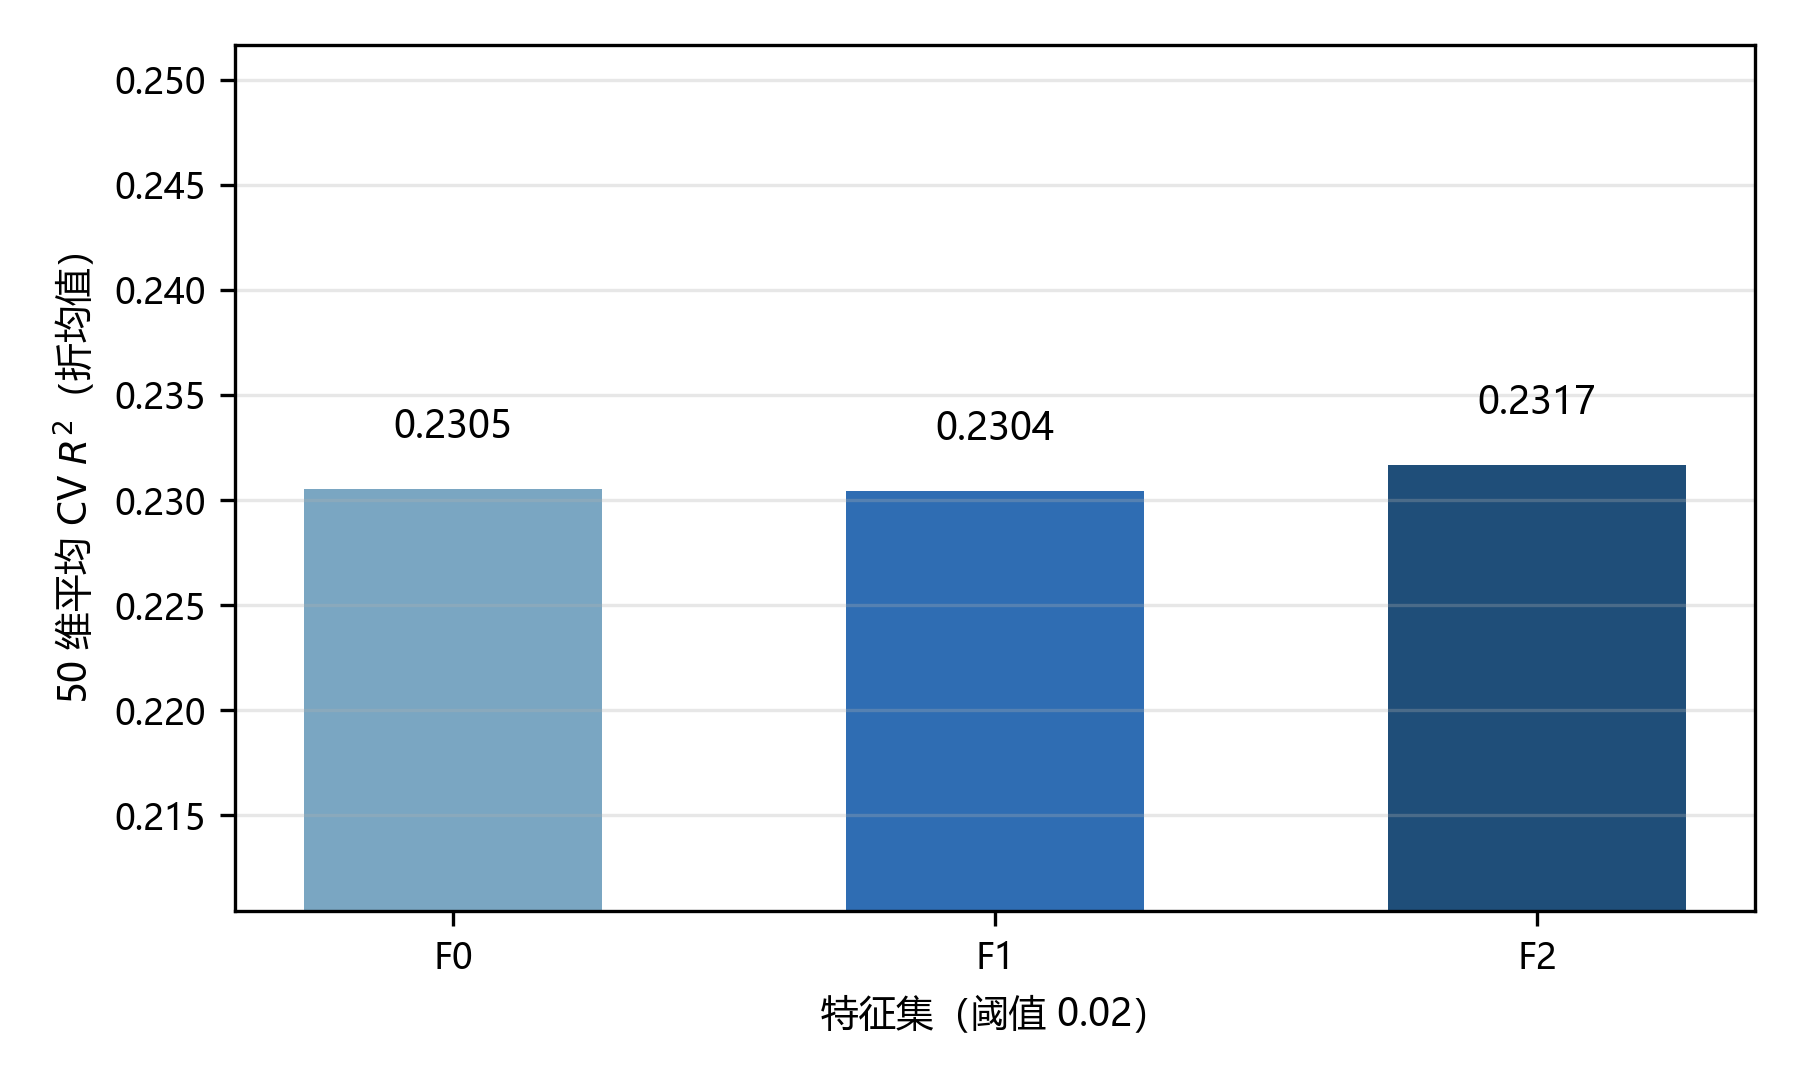
\includegraphics[width=0.64\textwidth]{图M3-02-特征集决策.png}
\caption{三套特征集在主模型下的平均交叉验证 $R^2$}
\label{fig:q1-featureset}
\end{figure}

图 \ref{fig:q1-featureset} 显示三根柱几乎等高：F2 比 F1 高 \textbf{0.0012}，F1 比 F0 低 \textbf{0.0001}。若只看“哪根柱最高”会选 F2，但预注册规则要求提升达到 \textbf{0.02} 才增加特征，因此最终采用 F0。这个结果说明，在本题的样本量下，追加 \textbf{4} 个聚合列与 \textbf{1} 个热量列没有带来可辨别的增益，保留更简的特征集反而降低了过拟合风险。

\subsubsection{逐维预测性能}

图 \ref{fig:q1-dim} 给出 \textbf{50} 个感官维度的逐维交叉验证 $R^2$，按降序排列并按香气、风味、其他三组着色。最高的是 \texttt{acetic} 的 \textbf{0.7234}，其次是 \texttt{acidity}、\texttt{alcohol}、\texttt{lactic} 和 \texttt{bitternes}；最低的是 \texttt{A\_hops\_tropical} 的 \textbf{-0.0854}，其后是 \texttt{F\_esters\_flower}、\texttt{F\_malt\_grain} 和 \texttt{A\_esters\_fruity}。前五个维度都与酸、醇、苦味等有明确化学对应的感官有关，后四个维度则更依赖品评员对细微香气的整体判断，化合物信息不足以稳定预测。

\begin{figure}[H]
\centering
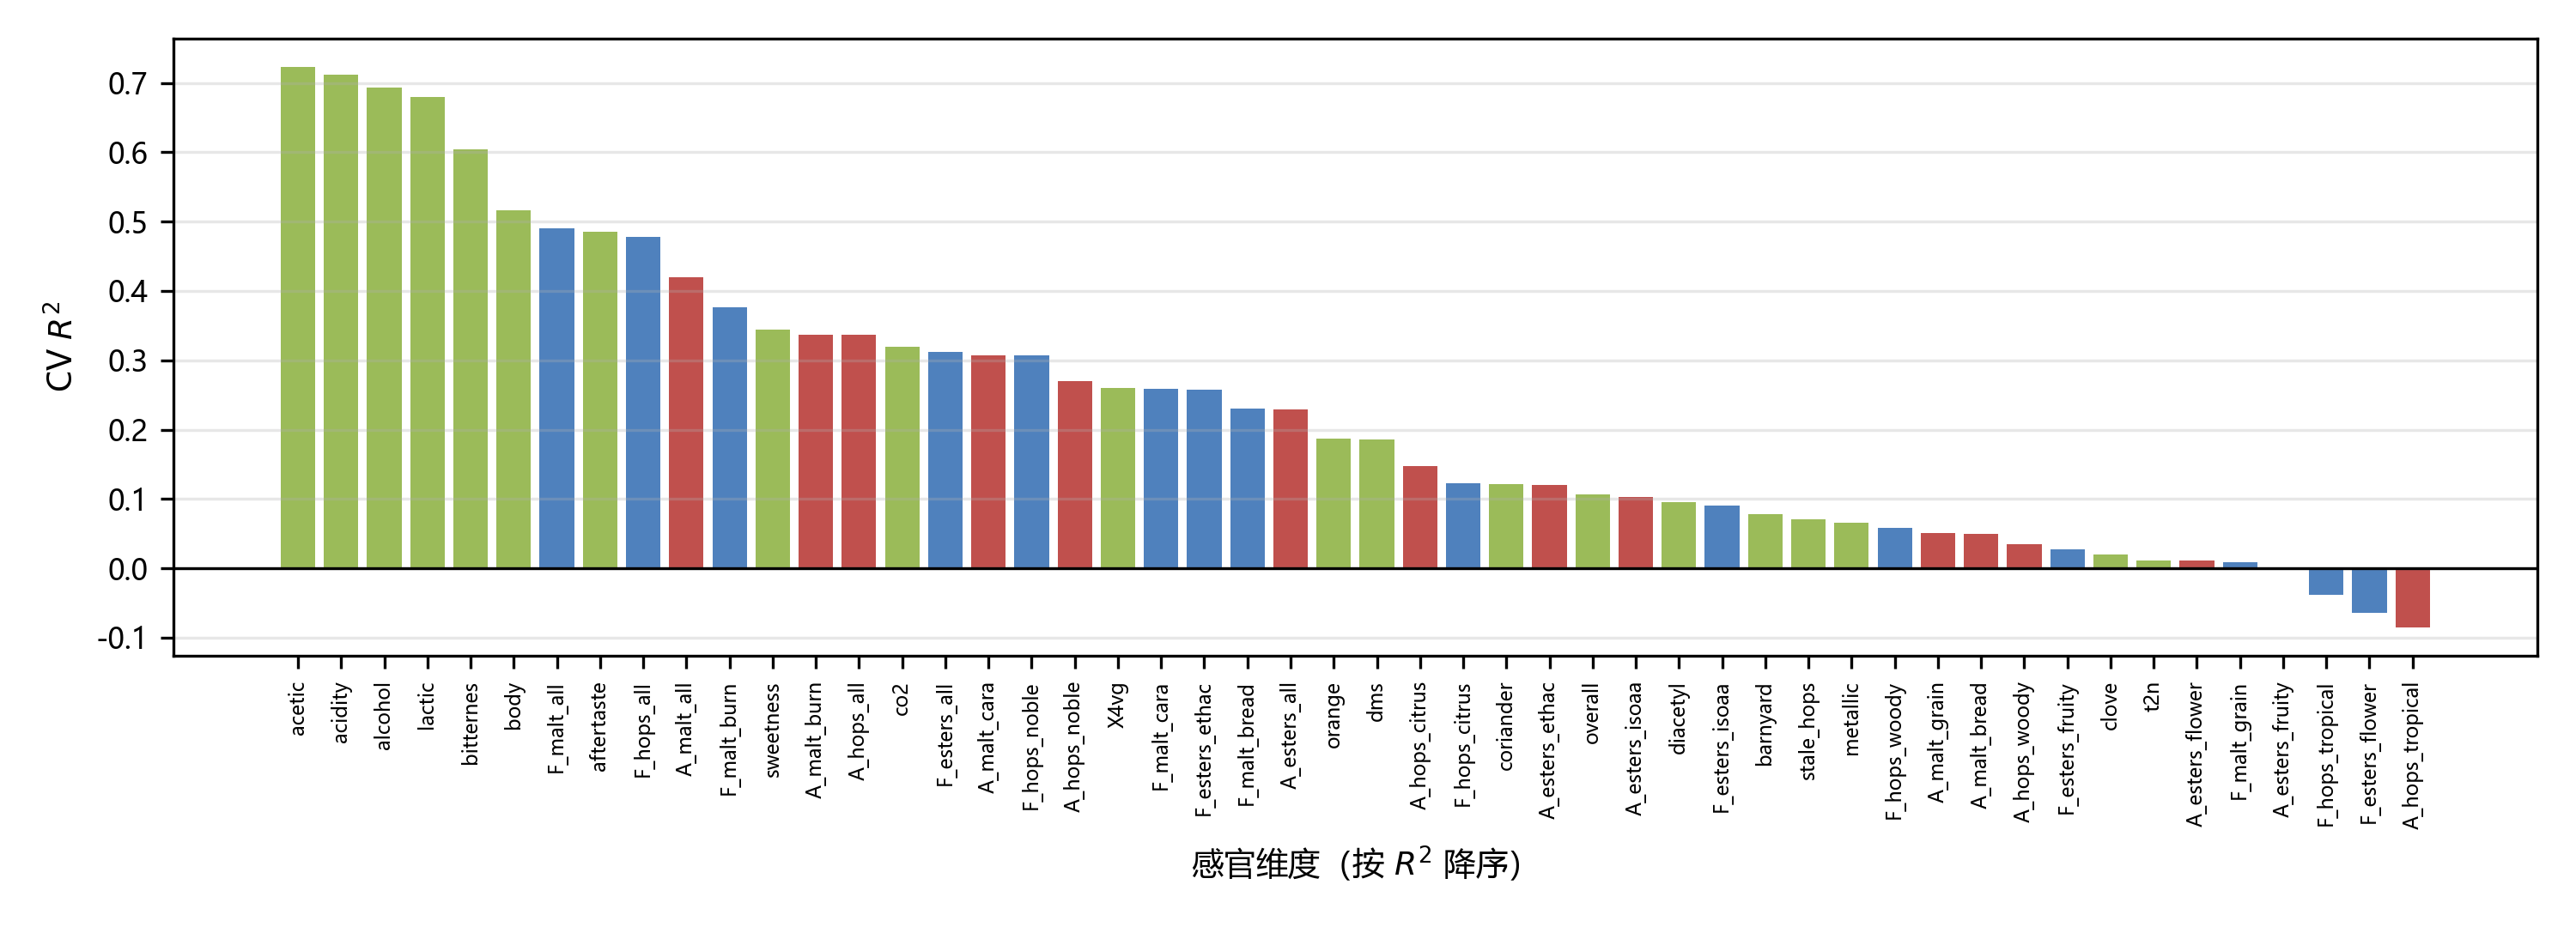
\includegraphics[width=0.96\textwidth]{图M3-03-逐维CV性能.png}
\caption{\textbf{50} 个感官维度的交叉验证 $R^2$（降序，按香气、风味、其他分组着色）}
\label{fig:q1-dim}
\end{figure}

逐维差异提示我们不要用“平均 $R^2$”掩盖结构性差异。平均 $R^2$ 为 \textbf{0.2305}，但 \textbf{50} 维中有的正值较高、有的接近零甚至为负；负值维度说明该维度的折外预测不如均值基线，本文如实保留，不删除、不单独调参。后文的 T7 信息损失与 T8 塌缩维，正是这种逐维差异在分级层面的表现。

\subsubsection{分级结果与可读口径}

把 OOF 连续预测送入 ALR 后，得到 \textbf{250}$\times$\textbf{50} 的评分表。主表的 \textbf{0} 级与 \textbf{6} 级整列为空，\textbf{5} 级只有 \textbf{23} 格，主要出现在 \texttt{bitternes}、\texttt{alcohol}、\texttt{aftertaste}、\texttt{body} 等维度；其余格子集中在 \textbf{1--4} 级。图 \ref{fig:q1-heat} 的逐维行归一化热图显示，不同维度的峰值位置不同，但两端都明显偏空。

\begin{figure}[H]
\centering
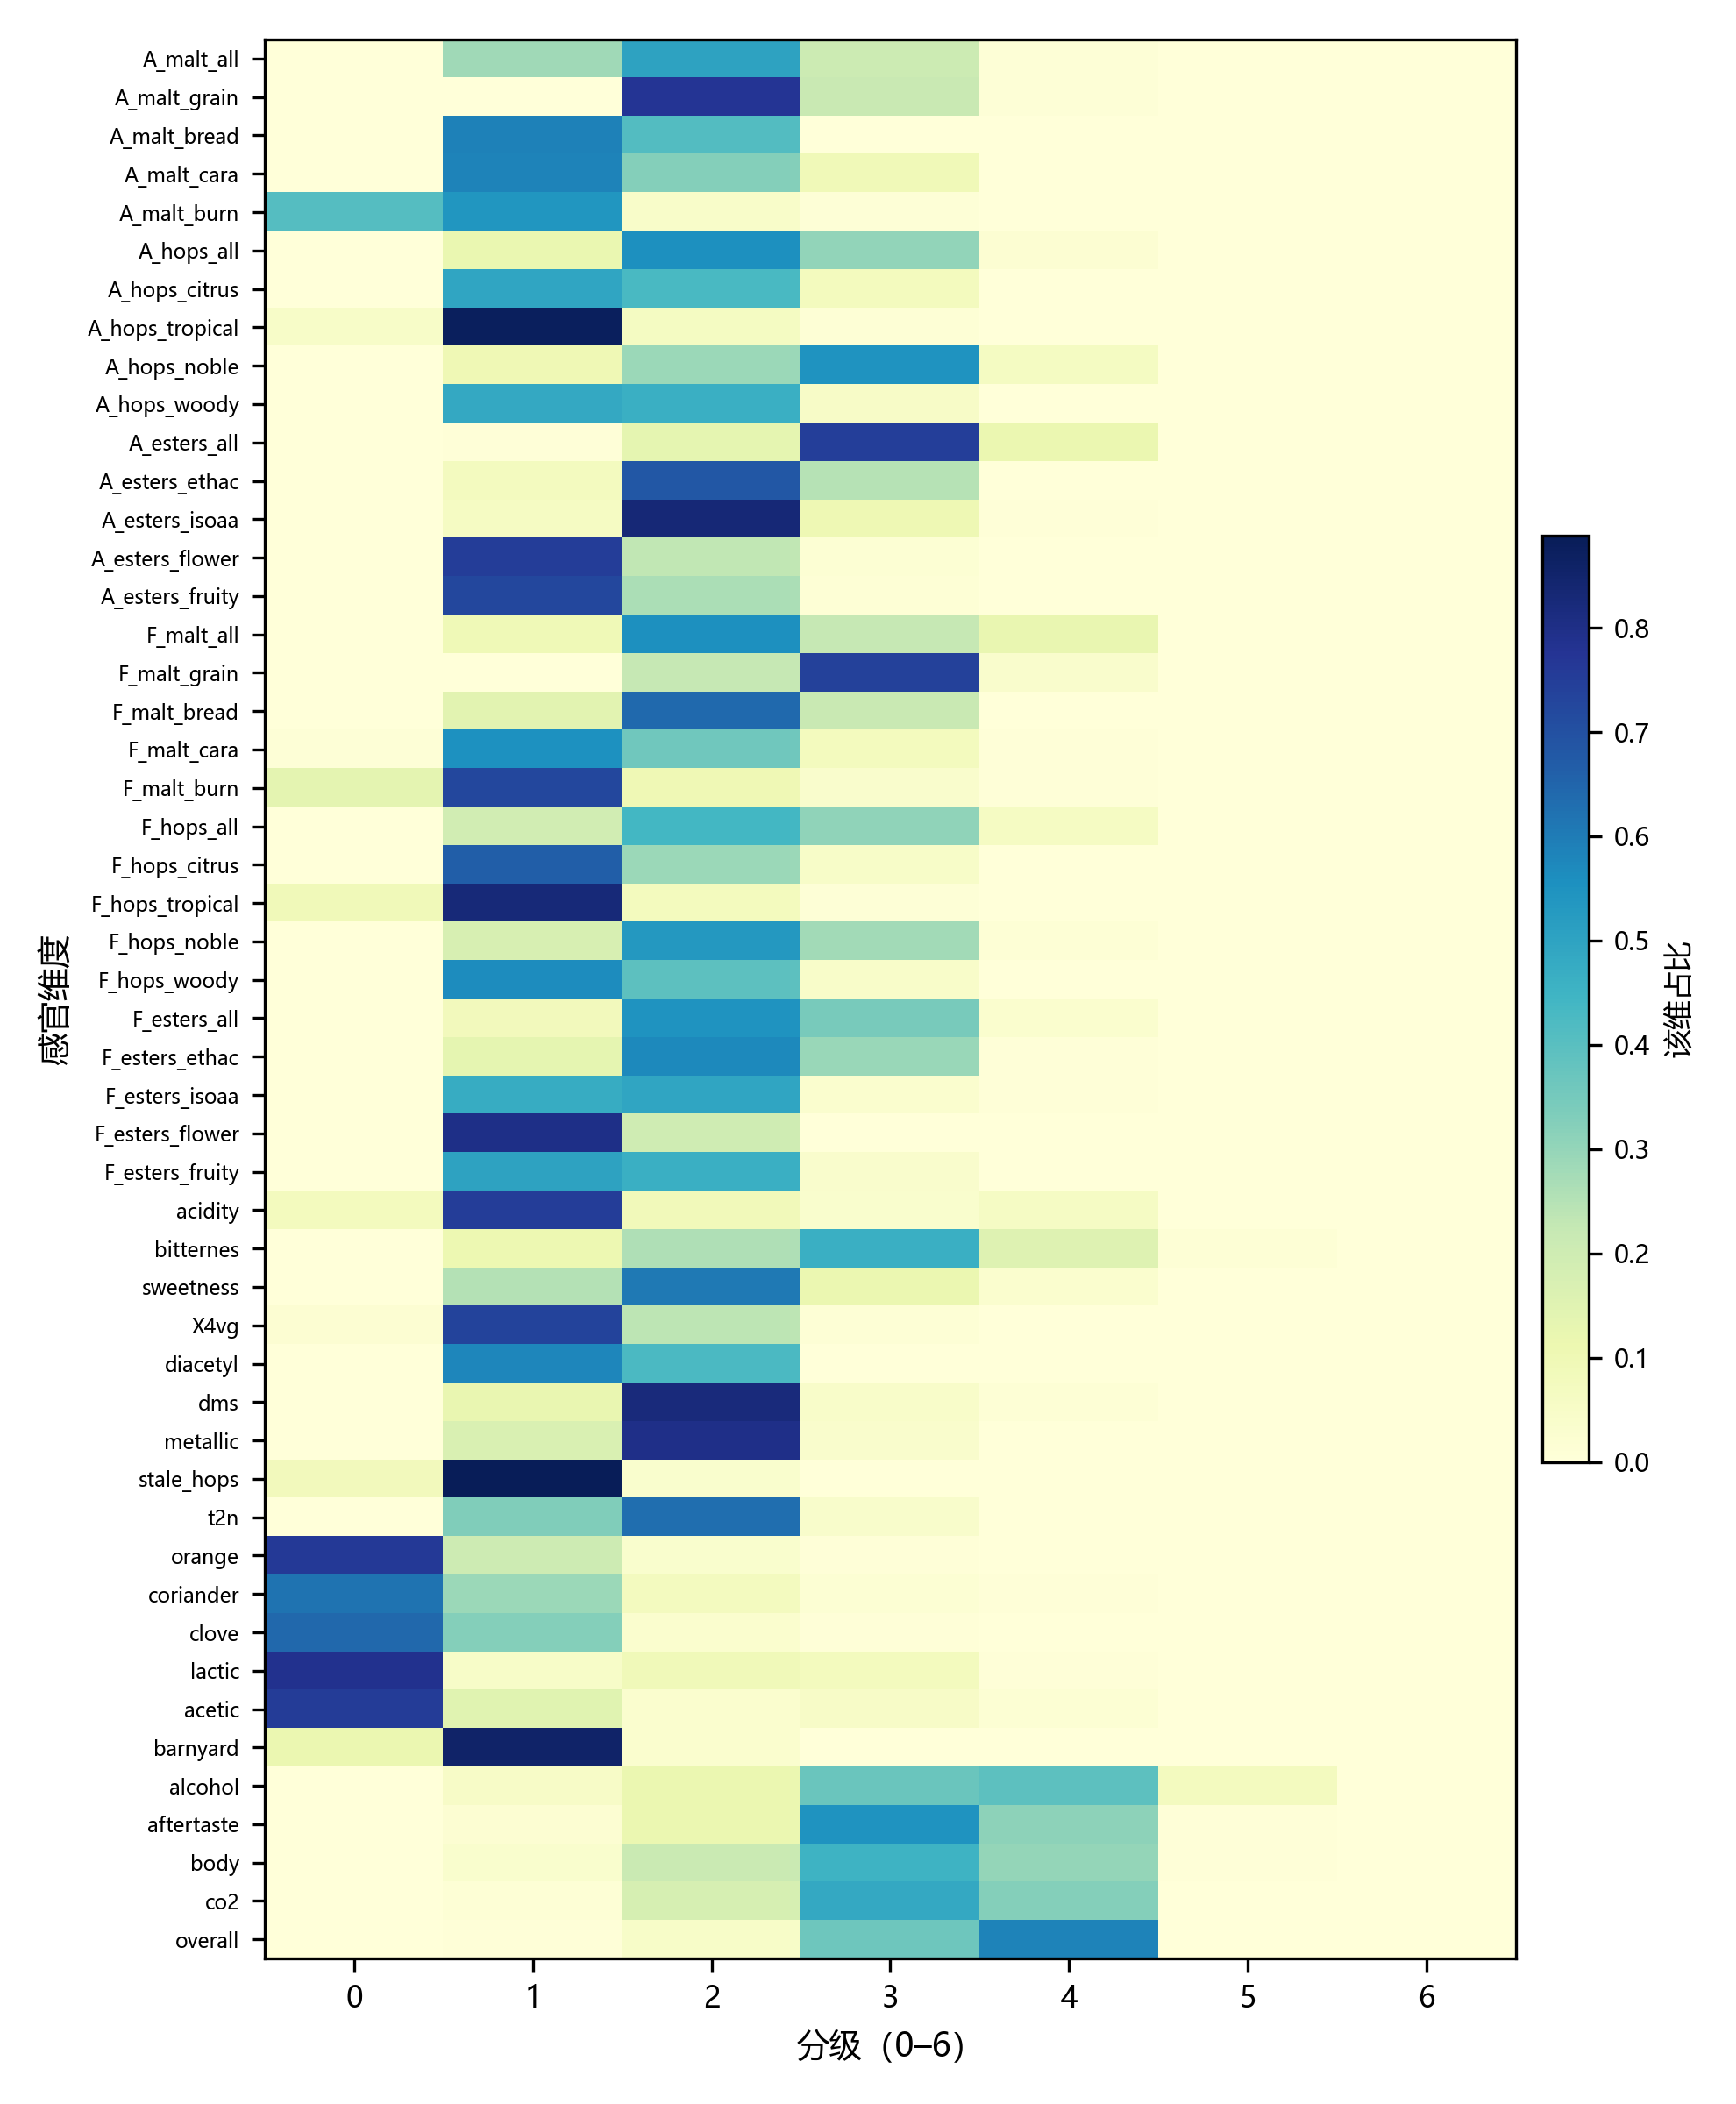
\includegraphics[width=0.56\textwidth]{图M3-04-分级分布热图.png}
\caption{主评分表 \textbf{50} 维 $\times$ \textbf{0--6} 七级的行归一化频数}
\label{fig:q1-heat}
\end{figure}

两端为空并不等于分级规则失效。T1 已证明 ALR 在规则定义域内是单调的，\textbf{50/50} 维都能在 \textbf{0--6} 的每一级取到平台；主表两端为空，是因为送入 ALR 的 OOF 预测本身值域收窄，而不是映射把两端“吃掉”了。下一小节把这个现象写成可检验的命题。

为便于按题面 \textbf{0--6} 阅读，本文另给一张可读口径辅助表。对第 $d$ 维，先把 OOF 预测做逐维单调仿射
\begin{equation}
\tilde y_d=\mu^{\mathrm{label}}_d+\left(\hat y_d-\mu^{\mathrm{pred}}_d\right)\cdot
\frac{\sigma^{\mathrm{label}}_d}{\sigma^{\mathrm{pred}}_d},
\label{eq:readable}
\end{equation}
其中 $\mu$、$\sigma$ 分别为标签与预测的均值、总体标准差；再把 $\tilde y_d$ 送入同一套 ALR 锚点。式 \eqref{eq:readable} 只改变刻度，不改变同一维度内的样本排序，因此辅助表与主表单调同序。辅助表的 \textbf{50} 维合计频数如表 \ref{tab:q1-readable} 所示，\textbf{7} 个等级全部出现，逆序对为 \textbf{0}。

\begin{table}[H]
\centering
\zihao{5}
\begin{tabularx}{\textwidth}{@{}l*{7}{r}rr@{}}
\toprule
口径 & \textbf{0} 级 & \textbf{1} 级 & \textbf{2} 级 & \textbf{3} 级 & \textbf{4} 级 & \textbf{5} 级 & \textbf{6} 级 & 合计 & 逆序对 \\
\midrule
可读口径 & \textbf{2945} & \textbf{3221} & \textbf{2634} & \textbf{2020} & \textbf{1183} & \textbf{412} & \textbf{85} & \textbf{12500} & \textbf{0} \\
\bottomrule
\end{tabularx}
\caption{可读口径辅助表的 \textbf{50} 维合计频数}
\label{tab:q1-readable}
\end{table}

表 \ref{tab:q1-readable} 的合计 \textbf{12500} 等于 \textbf{250}$\times$\textbf{50}。可读表与主表的同格率为 \textbf{55.9\%}，逐维 Spearman 在 \textbf{0.4168--0.9982} 之间；同格率不是 \textbf{100\%}，是因为式 \eqref{eq:readable} 把主表中并列的样本重新拉开，弱维的等级切点因此改变，但逆序对仍为 \textbf{0}，说明“同序”成立。缩放系数的算术平均为 \textbf{2.43}，逐维在 \textbf{1.31--3.55} 之间，量级与“预测标准差约为标签的 \textbf{0.444} 倍”一致。

\subsubsection{检验结果与刻度不可达命题}
\label{sec:q1-check}

T1--T8、E1--E3 与缺失鲁棒性的结果汇总在表 \ref{tab:q1-check}。其中 T2、T7、T8 三条不通过，本文不把它们归因于实现缺陷，而是统一写成\textbf{刻度不可达命题}：折外预测是条件均值，条件均值的方差天然小于标签方差；在近似线性、噪声与信号不相关的常见情形下，方差比 $\approx R^2$。实测逐维预测与标签的标准差之比平均为 \textbf{0.444}（范围 \textbf{0.281--0.763}），故方差比约为 $0.444^2\approx\textbf{0.197}$，与折均 $R^2$ 的 \textbf{0.2305}、OOF 全局 $R^2$ 的 \textbf{0.2565} 同阶。这个比例是 $R^2$ 小于 \textbf{1} 的直接影子，不是标定实现可以消除的偏差。

ALR 的锚点固定在标签的 \textbf{0.5\%} 与 \textbf{99.5\%} 分位数上。要得到 \textbf{6} 级，需 $s^{\ast}\ge 5.5$，即预测值至少位于锚点区间的 $5.5/6$ 处；在标签分布上，这大约对应第 \textbf{92} 百分位。一个标准差仅为标签 \textbf{0.444} 倍的预测器，要越过这一门槛的概率接近 \textbf{0}，因此主表 \textbf{6} 级为空是锚点冻结时的数学必然。\textbf{0} 级要求预测落入最低的窄带，收窄后的预测同样难以进入；\textbf{5} 级门槛在区间的 \textbf{75\%} 处，故只在少数维度出现少量格子。即 \textbf{0/6 级不可达}是口径的数学必然，而不是分级规则的实现缺陷。由同一命题可以读出三条检验的含义：

\begin{itemize}
\item \textbf{T2（保序一致）}：min Spearman 为 \textbf{0.6575}。ALR 规则本身单调（T1 的 \textbf{50/50} 维通过），T2 偏低来自标签在 \textbf{0} 级的大量并列，例如 \texttt{acetic} 有 \textbf{82.8\%} 的样本落在 \textbf{0} 级；并列越多，Spearman 的惩罚越重。
\item \textbf{T7（信息损失）}：min Spearman 为 \textbf{0.5470}。分级把连续预测压成少数等级，等级越少、并列越多，分级与连续预测的秩相关越低；这是离散化本身的信息损失，不是预测器换了目标。
\item \textbf{T8（塌缩维）}：实际使用等级数不超过 \textbf{3} 的维度有 \textbf{19} 个，其中 \textbf{3} 个维度只用了 \textbf{2} 级。原方案要求塌缩维不超过 \textbf{5}，该阈值与本方案冻结的标签锚点不相容；按同一锚点，收窄预测必然集中在中间等级。
\end{itemize}

\begin{table}[H]
\centering
\zihao{-5}
\begin{tabularx}{\textwidth}{@{}p{0.08\textwidth}p{0.20\textwidth}p{0.18\textwidth}p{0.16\textwidth}X@{}}
\toprule
编号 & 指标 & 实测 & 判据 & 结论与解释 \\
\midrule
T1 & 单调性（\textbf{50} 维） & \textbf{50/50} 通过 & 非降且 \textbf{0--6} 平台齐全 & 通过 \\
T2 & 保序一致 min Spearman & \textbf{0.6575} & $\ge 0.99$ & 不通过；刻度不可达（标签并列） \\
T3 & 参考分级等级数 & \textbf{45} 维 \textbf{7} 级、\textbf{5} 维 \textbf{6} 级 & min $\ge 5$ & 通过 \\
T4 & 边界确定性（\textbf{50} 维） & \textbf{50/50} 通过 & 六类输入一致 & 通过 \\
T5 & 往返复原 & \textbf{12500/12500} & $=1.0$ & 通过 \\
T6 & 锚点敏感性均值 & \textbf{0.8308}；P1/P99 为 \textbf{0.8890} & 只报告 & 记录 \\
T7 & 信息损失 min Spearman & \textbf{0.5470} & $\ge 0.95$ & 不通过；刻度不可达（离散损失） \\
T8 & 塌缩维 / 仅 \textbf{2} 级维 & \textbf{19} / \textbf{3} & 塌缩维 $\le 5$ & 不通过；刻度不可达（阈值冲突） \\
E1 & 有效格 / 化合物 & \textbf{949/2200}；\textbf{42} 个 & 平均绝对差 $\le 0.25$ & 通过；\textbf{0.1201}，方向一致率 \textbf{0.9968} \\
E2 & 感官协同结构 & \textbf{1225} 对；\textbf{0.1719} & 平均绝对差 $\le 0.20$ & 通过；方向一致率 \textbf{0.8098} \\
E3 & 独立方向证据 & \textbf{39} 映射 / \textbf{34} 有效 & $N_{\mathrm{eff}}\ge 20$ 且 $R_3\ge 0.60$ & 通过；$R_3=\textbf{0.9706}$ \\
鲁棒性 & 缺失 \textbf{20\%} & 折均 \textbf{0.2121}；一致率 \textbf{0.8882} & 记录 & 下降可控 \\
\bottomrule
\end{tabularx}
\caption{问题一的检验、独立证据与缺失鲁棒性汇总}
\label{tab:q1-check}
\end{table}

表 \ref{tab:q1-check} 的 T2、T7、T8 三行都应在“刻度不可达命题”下阅读：T2 是标签并列造成的秩相关下降，T7 是离散化造成的信息损失，T8 是阈值与冻结锚点不相容。三者都不是“换一个模型就能变好”的执行问题；若强行拉伸预测去填满 \textbf{0} 级与 \textbf{6} 级，反而会破坏锚点语义，让评分表与连续预测不再同序。本文的选择是保留主表、如实登记，并用可读口径辅助表解决“看起来没有 \textbf{6} 级”的阅读问题。

\subsubsection{独立证据与缺失鲁棒性}

缺失鲁棒性通过人工遮蔽测试折的 \textbf{5\%}、\textbf{10\%}、\textbf{20\%} 个格子来检验。折均 $R^2$ 从 \textbf{0.2305} 降到 \textbf{0.2266}、\textbf{0.2256}、\textbf{0.2121}，分级一致率从 \textbf{1.0000} 降到 \textbf{0.9658}、\textbf{0.9348}、\textbf{0.8882}。图 \ref{fig:q1-mask} 的左图是 $R^2$ 的下降曲线，右图是一致率曲线；两条曲线在 \textbf{10\%} 以内都比较平，到 \textbf{20\%} 才明显下弯，说明模型对偶发缺失有缓冲，但不适合在缺失率很高时直接使用。

\begin{figure}[H]
\centering
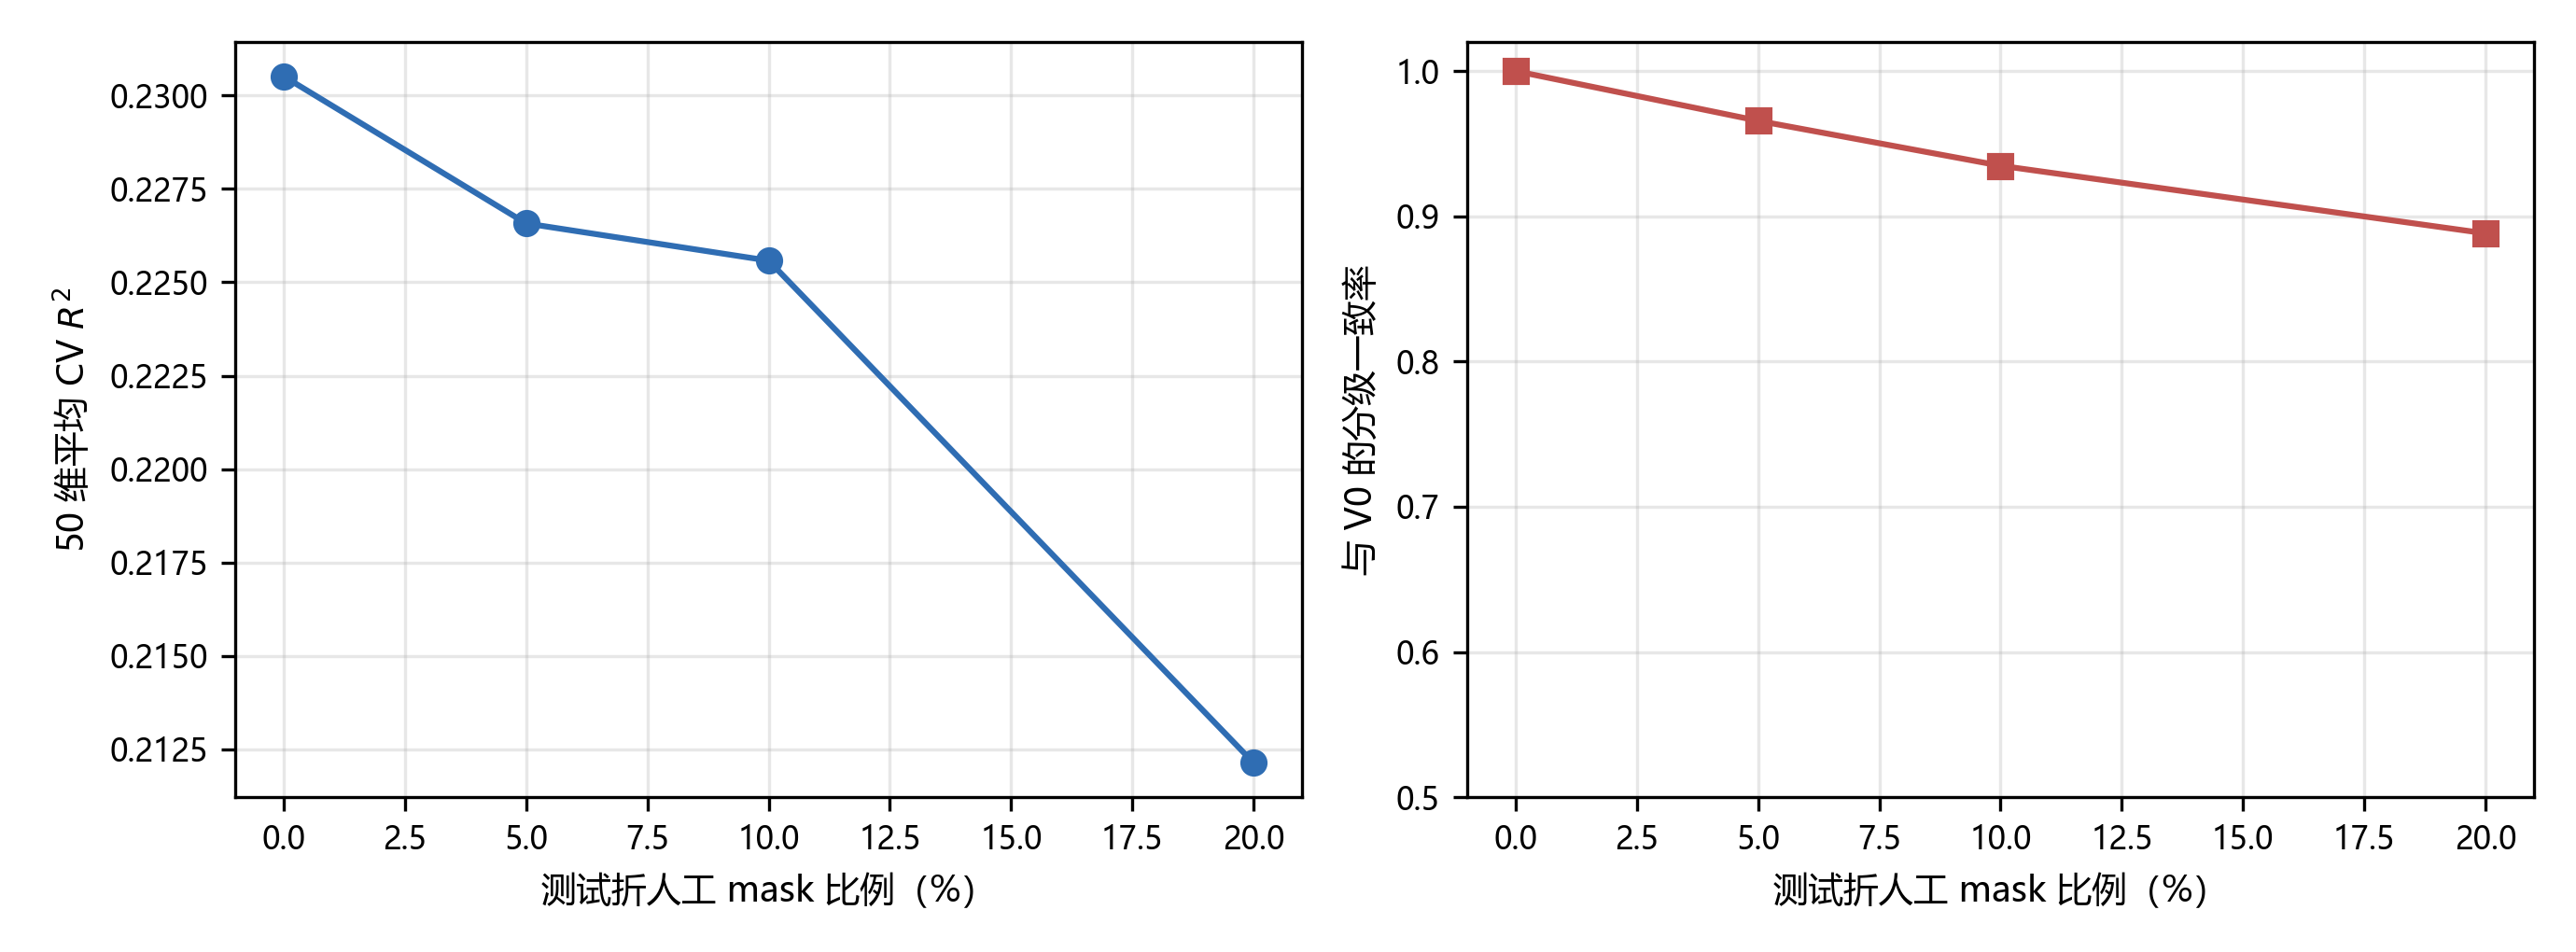
\includegraphics[width=0.92\textwidth]{图M3-05-缺失鲁棒性.png}
\caption{人工缺失比例对折均 $R^2$ 与分级一致率的影响}
\label{fig:q1-mask}
\end{figure}

E1 用 \texttt{6.csv} 的参考相关核对 OOF 预测重算的相关结构。\texttt{6.csv} 有 \textbf{44} 个指标，其中 \textbf{42} 个能映射到 \texttt{1.csv}；在 \textbf{2200} 个格子里有 \textbf{949} 个有效格，平均绝对差为 \textbf{0.1201}，方向一致率为 \textbf{0.9968}。图 \ref{fig:q1-e1} 的散点沿对角线分布，说明预测重算的相关方向与题方参考相关基本一致；偏离主要出现在参考相关接近 \textbf{0} 的格子，此时方向本身不稳定。

\begin{figure}[H]
\centering
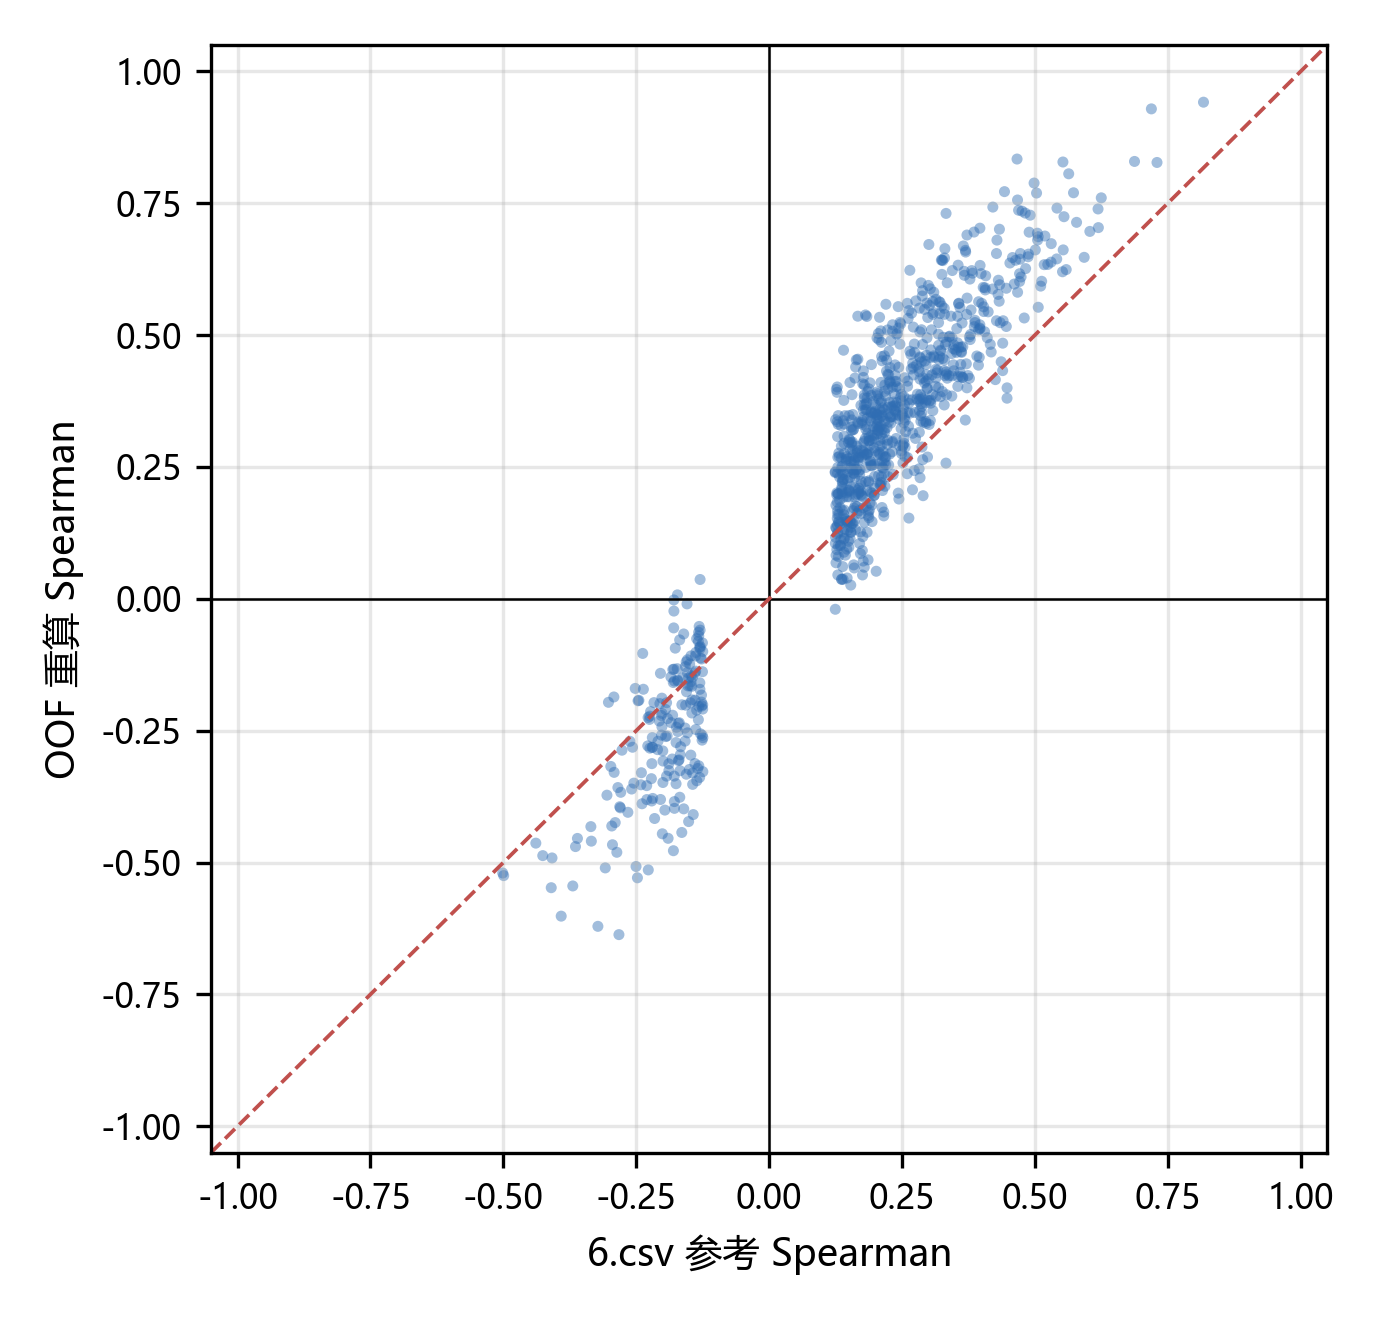
\includegraphics[width=0.46\textwidth]{图M3-06-E1方向散点.png}
\caption{题方 \texttt{6.csv} 参考 Spearman 与 OOF 重算 Spearman 的逐格对照}
\label{fig:q1-e1}
\end{figure}

E2 用 \texttt{5.csv} 的 \textbf{50}$\times$\textbf{50} 感官相关阵核对预测矩阵的列间结构，\textbf{1225} 对的平均绝对差为 \textbf{0.1719}，方向一致率为 \textbf{0.8098}，低于 E1 但仍在判据内；这说明模型不仅拟合了单维均值，也保留了一部分感官维度之间的协同结构。E3 把 \texttt{7.csv} 的 \textbf{186} 个属性桥接到感官维度，得到 \textbf{39} 个可映射属性、\textbf{34} 个有效映射，方向一致率 $R_3$ 为 \textbf{0.9706}，说明预测方向与独立属性证据一致。

\subsubsection{小结}

问题一的主线可以概括为“随机森林拟合连续评分、ALR 转成等级、刻度不可达命题解释两端为空”。主模型在 OOF 全局口径下为 \textbf{0.2565}，折均口径下为 \textbf{0.2305}，都高于同口径基线；逐维差异、T2/T7/T8 的偏离、E1--E3 的独立证据与缺失鲁棒性共同说明：模型在平均意义上有效，在弱维和两端等级上存在结构性限制。可读口径辅助表在不改变主表排序的前提下补足 \textbf{7} 级覆盖，为后续展示与使用提供了更友好的界面。

\section{问题二：共表达网络与关键化合物识别}

\subsection{问题描述}

问题二给出 \texttt{2.csv} 的化合物相关矩阵，要求建立共表达网络，并结合 \texttt{1.csv} 的化学特征与 \texttt{4.csv} 的感官标签，为每个感官维度给出 \textbf{3} 个关键化合物；同时要回答三个追问：排序是否稳定、结果是否有化学合理性、它与全局重要度排序是否一致。

这一问的输出不是一张“化合物重要性排行榜”，而是 \textbf{50} 个维度各自的 \textbf{3} 个化合物。若只按“化合物与感官维度的相关系数”排序，容易同时选中几个高度共线的同源化合物；若只按“网络中度数”排序，又会选出与感官目标无关的枢纽节点。本文把两种信息写成可加融合分，把图结构作为平滑项，并要求融合后的排序在重采样下可复核。

\subsection{模型建立}

\subsubsection{共表达图的构建}

把 \texttt{2.csv} 的 \textbf{231} 个节点剔除 \textbf{4} 个聚合列与 \textbf{1} 个热量列，保留 \textbf{226} 个候选化合物。对任意两个不同节点 $i,j$，令 $\rho_{ij}$ 为 \texttt{2.csv} 中的 Spearman 相关系数；当
\begin{equation}
\left|\rho_{ij}\right|\ge \tau
\label{eq:edge}
\end{equation}
时连一条无向边，边权取 $w_{ij}=|\rho_{ij}|$。阈值 $\tau$ 取 \textbf{0.30}。这个取值不是凭经验拍的：按 \textbf{226} 个节点共有 \textbf{25425} 个无序对、标称样本量 \textbf{250} 做 Fisher 变换，Bonferroni 校正后的单对临界值约为 \textbf{0.293754}，向上取整到 \textbf{0.30}\cite{benjamini1995}。在该阈值下，单对最大 $p$ 值仍小于校正后的显著性水平，图不会把大量噪声边纳入。

\subsubsection{直接相关得分与图平滑得分}

对化合物 $c$ 与感官维度 $d$，直接相关得分定义为
\begin{equation}
s_{\mathrm{direct}}(c,d)=\left|\mathrm{Spearman}\left(x_c,y_d\right)\right|,
\label{eq:sdirect}
\end{equation}
其中 $x_c$ 为 \texttt{1.csv} 中化合物 $c$ 的列，$y_d$ 为 \texttt{4.csv} 中第 $d$ 维标签；按列内可用样本成对计算，不插补。$s_{\mathrm{direct}}$ 衡量“这个化合物自己与感官维度有多强的关系”，但它看不见邻居。

设化合物 $c$ 的邻居集合为 $N(c)=\{j\ne c:|\rho_{cj}|\ge\tau\}$，图平滑得分定义为邻居得分的加权平均：
\begin{equation}
s_{\mathrm{graph}}(c,d)=\frac{\sum_{j\in N(c)}w_{cj}\,s_{\mathrm{direct}}(j,d)}
{\sum_{j\in N(c)}w_{cj}}.
\label{eq:sgraph}
\end{equation}
式 \eqref{eq:sgraph} 的含义是：如果一个化合物自己与感官维度的相关不算最强，但它的邻居们都与该维度强相关，那么它仍可能是该维度的关键化合物。若邻居的 $s_{\mathrm{direct}}$ 缺失，则从分子分母同时剔除并重新归一化；若邻域为空，则回退到 $s_{\mathrm{direct}}$，保证每个节点都有得分。

\subsubsection{融合分数与 Top-3}

把两种得分按图项权重 $\lambda$ 融合：
\begin{equation}
\mathrm{score}(c,d)=(1-\lambda)\,s_{\mathrm{direct}}(c,d)+
\lambda\,s_{\mathrm{graph}}(c,d),
\label{eq:score}
\end{equation}
其中 $\lambda=\textbf{0.70}$，在结果产生之前预注册。对每个维度 $d$，按 $\mathrm{score}(c,d)$ 降序取前 \textbf{3} 个化合物；分数并列时按节点名的 ASCII 升序稳定排序。$\lambda=0$ 时融合分退化为直接相关，$\lambda=1$ 时退化为纯图平滑；本文把 $\lambda=0$ 作为对照，用来判断图项是否真的改变了排序。

\subsubsection{稳定性、化学合理性与全局对照}

稳定性用有放回重采样衡量：每次从 \textbf{250} 个 beer 行中有放回抽 \textbf{250} 行，重算 $s_{\mathrm{direct}}$ 与 $s_{\mathrm{graph}}$，按同一 $\tau$、$\lambda$ 重排，记录全样本第 $k$ 名化合物进入该维 Top-3 的频率。重复 \textbf{200} 次，随机种子为 \textbf{20261024}，图结构固定为题方 \texttt{2.csv}，只传播样本抽样不确定性。频率越高，说明该化合物在该维 Top-3 中的位置越不依赖具体样本。

化学合理性用“化合物来源品类”与“感官维度品类”的对应关系核对。对每个 Top-3 化合物，经名称对齐表桥接到 \texttt{8.xlsx} 的 \texttt{origin\_paper}，再与维度在 \texttt{Sensory names} 中的 \texttt{Category} 比较；两者相同记为一致，不同记为不一致，化合物或维度属于 Spices、Internal standard solution 或缺失品类时记为不可比。不可比项从一致率分母剔除，不并入不一致。

全局对照使用 \texttt{8.xlsx} 的 GBM 重要度表。该表只有 \textbf{231} 个化合物的全局重要度，没有逐感官维度的列，因此只能做全局层面的旁证，不能做逐维对照；这一点在结果中会明确标注。

\subsection{算法求解}

\subsubsection{建图与打分流程}

求解按以下顺序执行：读取 \texttt{2.csv}，按候选池剔除 \textbf{5} 个聚合/热量节点；按式 \eqref{eq:edge} 建无向图并统计节点数、边数、度分布与连通分量；读取 \texttt{1.csv} 与 \texttt{4.csv}，按 \texttt{beer} 对齐后逐对计算 $s_{\mathrm{direct}}$；对每个节点按式 \eqref{eq:sgraph} 计算邻居加权得分；按式 \eqref{eq:score} 融合并取 Top-3；最后做 \textbf{200} 次 bootstrap、\textbf{5} 组稳健性扰动与品类一致性核对。

计算量主要来自 $s_{\mathrm{direct}}$ 的 \textbf{226}$\times$\textbf{50} 个成对秩相关和 \textbf{200} 次重采样。每次重采样都要重算 \textbf{226}$\times$\textbf{50} 的相关矩阵，但图结构不变，邻居与边权可以复用；因此总耗时由相关计算主导，而不是由建图主导。这个设计使得 \textbf{200} 次 bootstrap 在普通工作站上可以在可接受时间内完成。

\subsubsection{稳定性与扰动设计}

稳定性只重采样样本行，不重采样图结构。原因是题方给出的 \texttt{2.csv} 是固定的相关矩阵，若把图结构也纳入重采样，就会把“题方提供的图”与“样本抽样”两种不确定性混在一起，无法判断频率下降来自哪一类。本文把图结构固定，让 bootstrap 频率只回答“换一批样本，Top-3 会不会变”。

稳健性另设 \textbf{5} 组扰动：把 $\tau$ 调到 \textbf{0.25} 与 \textbf{0.35}，去掉负边只保留正边，把 $\lambda$ 调到 \textbf{0.30} 与 \textbf{0.50}。每组扰动都重算 Top-3，并与主口径的 Top-3 计算逐维 Jaccard 系数，再取 \textbf{50} 维平均。Jaccard 定义为两个集合的交集大小除以并集大小；它比“重合个数除以 3”更严格，因为分母会随两个集合的并集变化。

\subsection{求解结果}

\subsubsection{共表达图的结构}

按 $\tau=0.30$ 建图后，网络含 \textbf{226} 个节点、\textbf{3758} 条边，其中正边 \textbf{3362} 条、负边 \textbf{396} 条；密度为 \textbf{0.147807}，平均度为 \textbf{33.2566}，孤立点 \textbf{4} 个，连通分量 \textbf{5} 个，最大连通分量含 \textbf{222} 个节点。负边按绝对值计入边权，因为本文关心的是关联强度而不是方向；正边-only 的情形留作稳健性检查。

\begin{figure}[H]
\centering
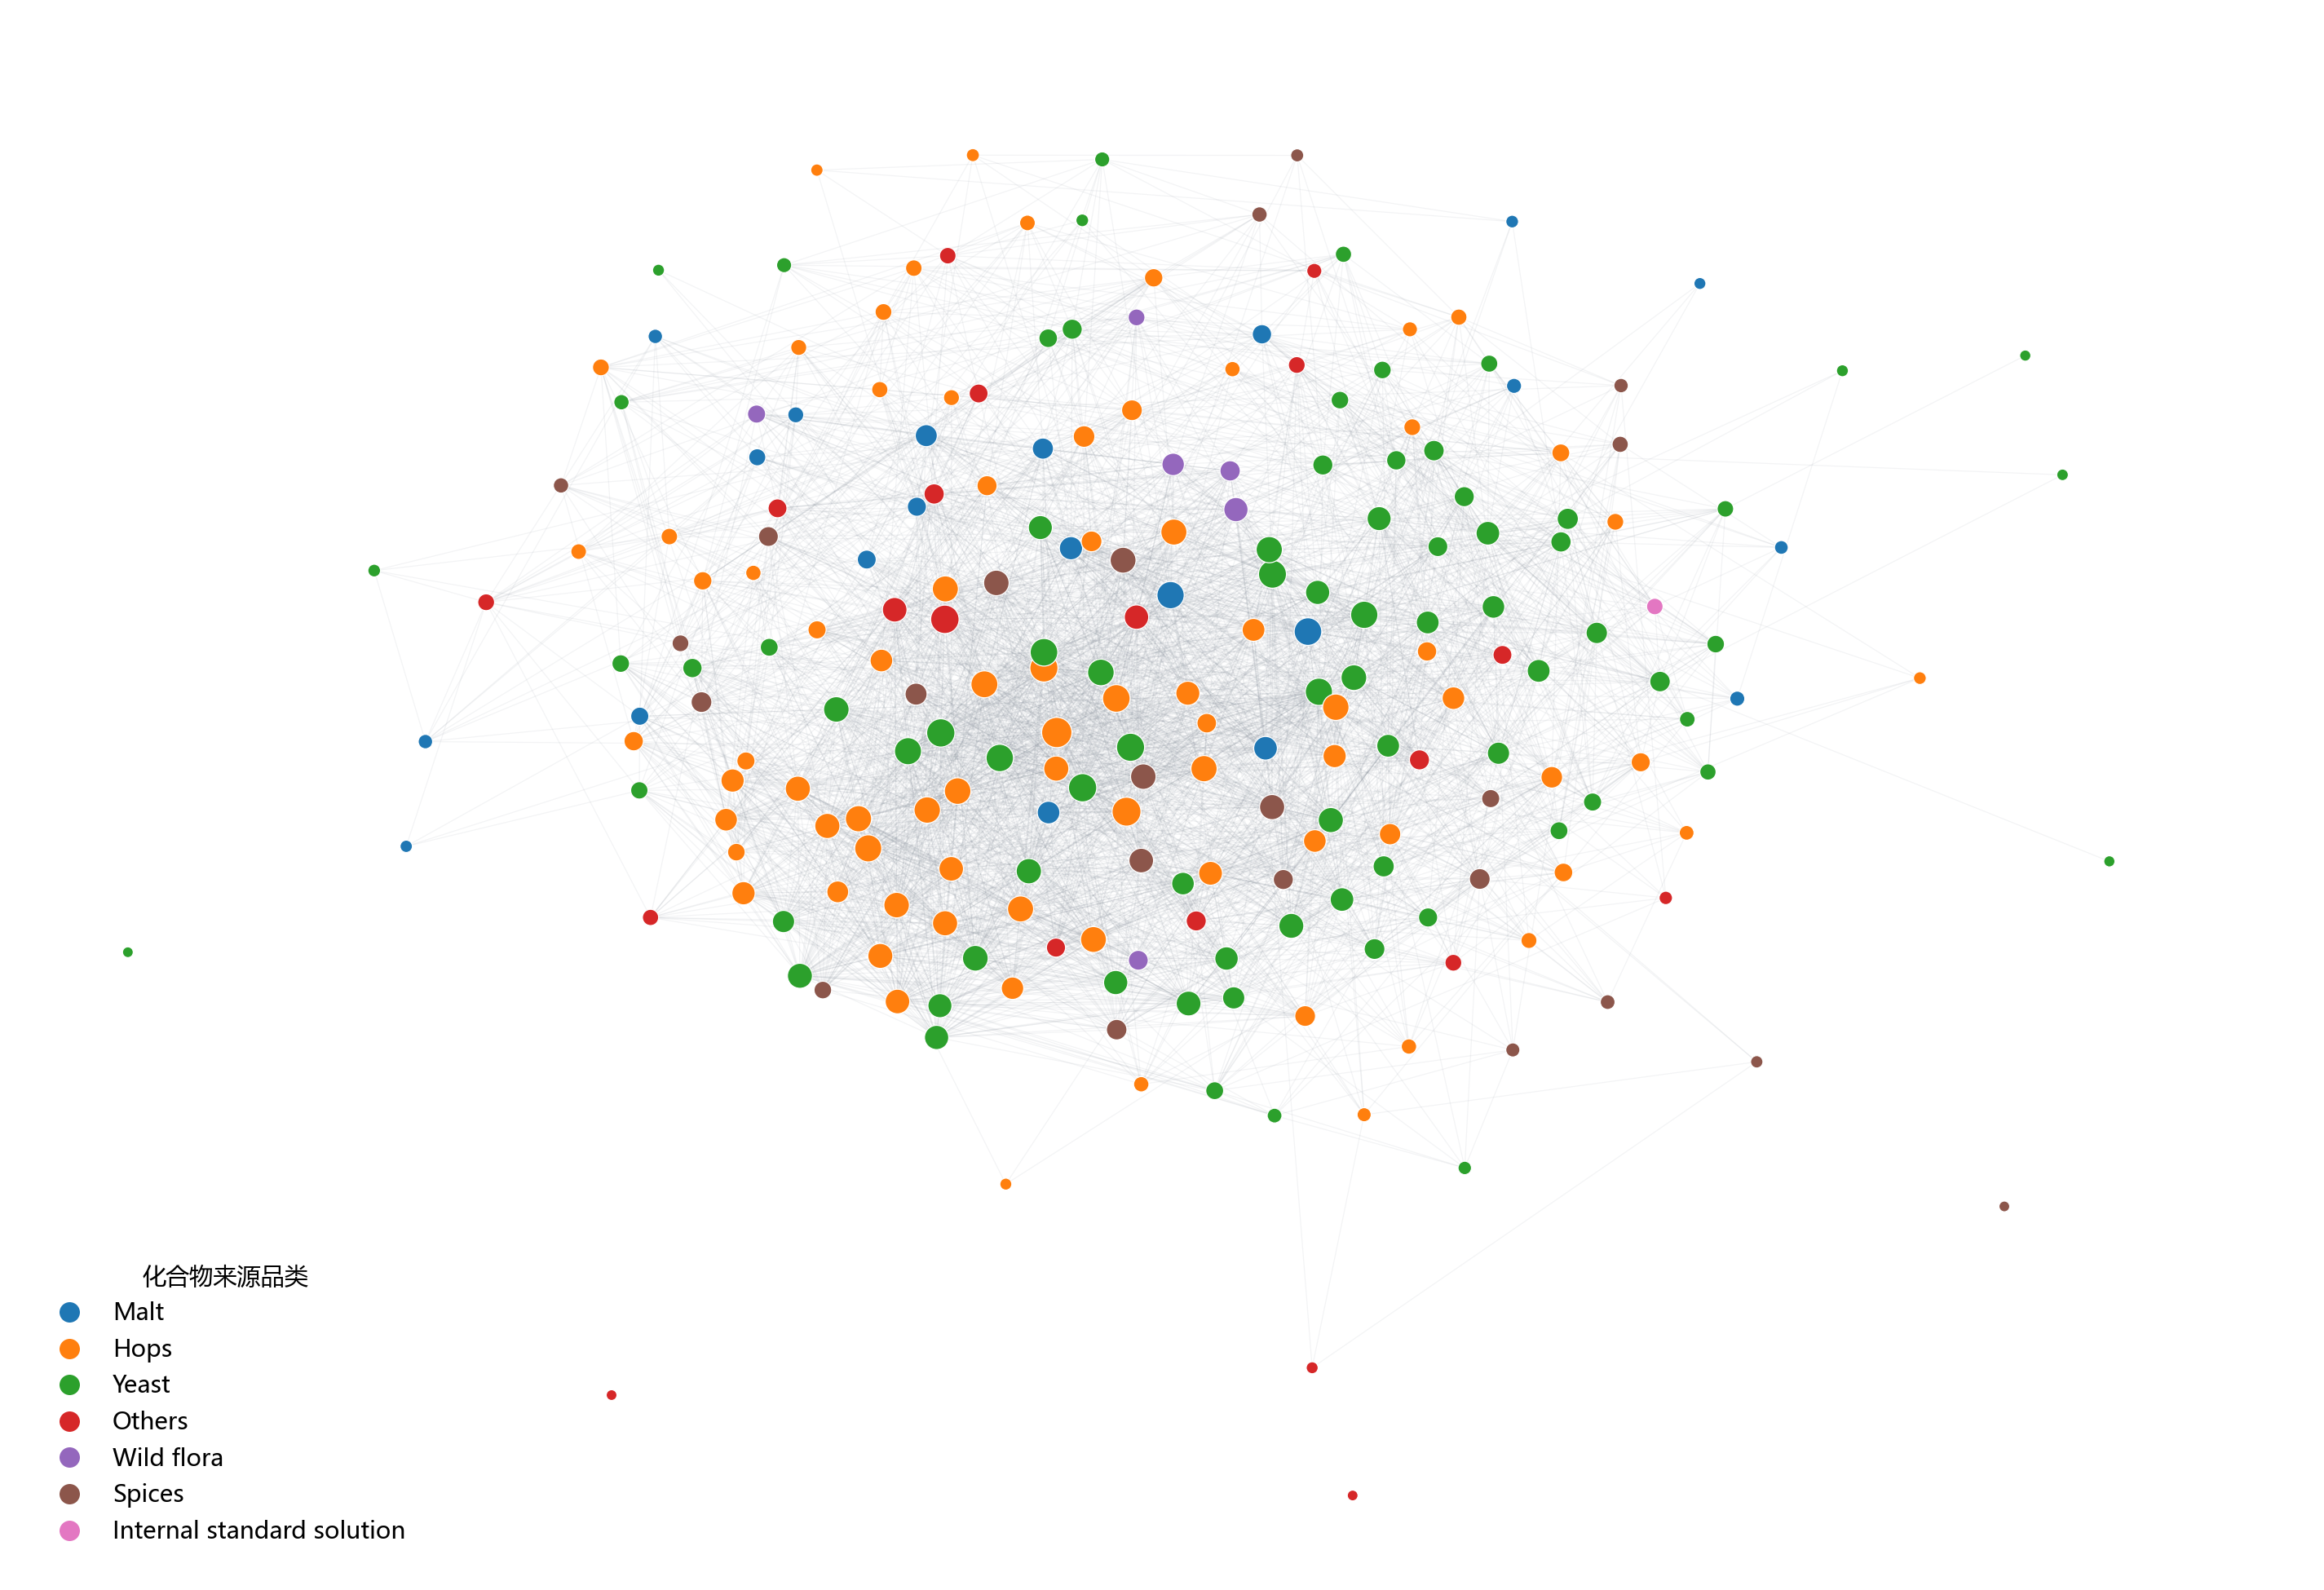
\includegraphics[width=0.88\textwidth]{图M2-01-共表达网络.png}
\caption{化合物共表达网络（边阈值 \textbf{0.30}，边权为 $|\rho|$；节点颜色表示来源品类，节点大小表示连接度）}
\label{fig:q2-network}
\end{figure}

图 \ref{fig:q2-network} 显示网络主体是一个大分量，外围有少量度较低的节点和 \textbf{4} 个孤立点。节点颜色把 Malt、Hops、Yeast、Others、Wild flora、Spices 等来源品类混在一起，说明同一来源的化合物并不总是聚成一团；这也解释了后文品类一致率不可能很高：网络连接由相关结构决定，而不是由来源标签决定。

\subsubsection{Top-3 关键化合物}

表 \ref{tab:q2-top3} 列出 \textbf{8} 个代表性维度的 Top-3 及 bootstrap 入选频率。选择这 \textbf{8} 个维度时，本文兼顾了麦芽、酒花、酯香、酸、苦、醇和整体感七个方向，并保留一个不可比维度 \texttt{overall}，用来看品类核对在缺失品类时的行为。

\begin{table}[H]
\centering
\zihao{-5}
\setlength{\tabcolsep}{4pt}
\begin{tabularx}{\textwidth}{@{}p{0.15\textwidth}p{0.22\textwidth}p{0.22\textwidth}p{0.22\textwidth}p{0.10\textwidth}@{}}
\toprule
感官维度 & 第 \textbf{1} 名（频率） & 第 \textbf{2} 名（频率） & 第 \textbf{3} 名（频率） & 维度品类 \\
\midrule
\texttt{A\_malt\_all} & Color（\textbf{0.975}） & Methylpyrazine（\textbf{0.760}） & Protein（\textbf{0.420}） & Malt \\
\texttt{A\_hops\_citrus} & Citronellol（\textbf{0.625}） & Humulene epoxide II（\textbf{0.290}） & Carbon dioxide（\textbf{0.345}） & Hops \\
\texttt{A\_esters\_ethac} & Ethyl propionate（\textbf{0.760}） & Phenethyl alcohol（\textbf{0.680}） & Acetaldehyde（\textbf{0.320}） & Yeast \\
\texttt{F\_malt\_bread} & Betaglucan（\textbf{0.665}） & Acetaldehyde（\textbf{0.840}） & Isobutanol（\textbf{0.285}） & Malt \\
\texttt{F\_esters\_ethac} & Ethyl propionate（\textbf{0.880}） & Ethyl acetate（\textbf{0.730}） & Acetaldehyde（\textbf{0.420}） & Yeast \\
\texttt{acidity} & Acetic acid（\textbf{0.940}） & pH（\textbf{0.550}） & 4-ethyl-phenol（\textbf{0.425}） & Others \\
\texttt{bitternes} & Iso-alpha acids（\textbf{0.815}） & Ethyl octanoate（\textbf{0.660}） & Dimethyl sulfide（\textbf{0.480}） & Others \\
\texttt{alcohol} & Ethanol（\textbf{1.000}） & Acetaldehyde（\textbf{0.900}） & Isobutanol（\textbf{0.550}） & Yeast \\
\bottomrule
\end{tabularx}
\caption{代表性感官维度的 Top-3 关键化合物与 bootstrap 入选频率}
\label{tab:q2-top3}
\end{table}

表 \ref{tab:q2-top3} 的第 \textbf{1} 名频率普遍高于第 \textbf{3} 名，例如 \texttt{alcohol} 的 Ethanol 为 \textbf{1.000}，\texttt{acidity} 的 Acetic acid 为 \textbf{0.940}，\texttt{F\_esters\_ethac} 的 Ethyl propionate 为 \textbf{0.880}；而 \texttt{A\_hops\_citrus} 的第 \textbf{2} 名只有 \textbf{0.290}，说明该维度的后位排序对样本扰动更敏感。这个差别与后文的整体稳定性结论一致：Top-1 较稳，Top-3 的后两位不稳。

\subsubsection{稳定性}

\textbf{200} 次 bootstrap 的 rank1、rank2、rank3 平均入选频率分别为 \textbf{0.6734}、\textbf{0.4896}、\textbf{0.3611}。在 \textbf{150} 个格子（\textbf{50} 维 $\times$ \textbf{3} 名次）中，频率不低于 \textbf{0.80} 的有 \textbf{22} 格，不低于 \textbf{0.50} 的有 \textbf{72} 格，低于 \textbf{0.50} 的有 \textbf{78} 格，最小值为 \textbf{0.125}。

\begin{figure}[H]
\centering
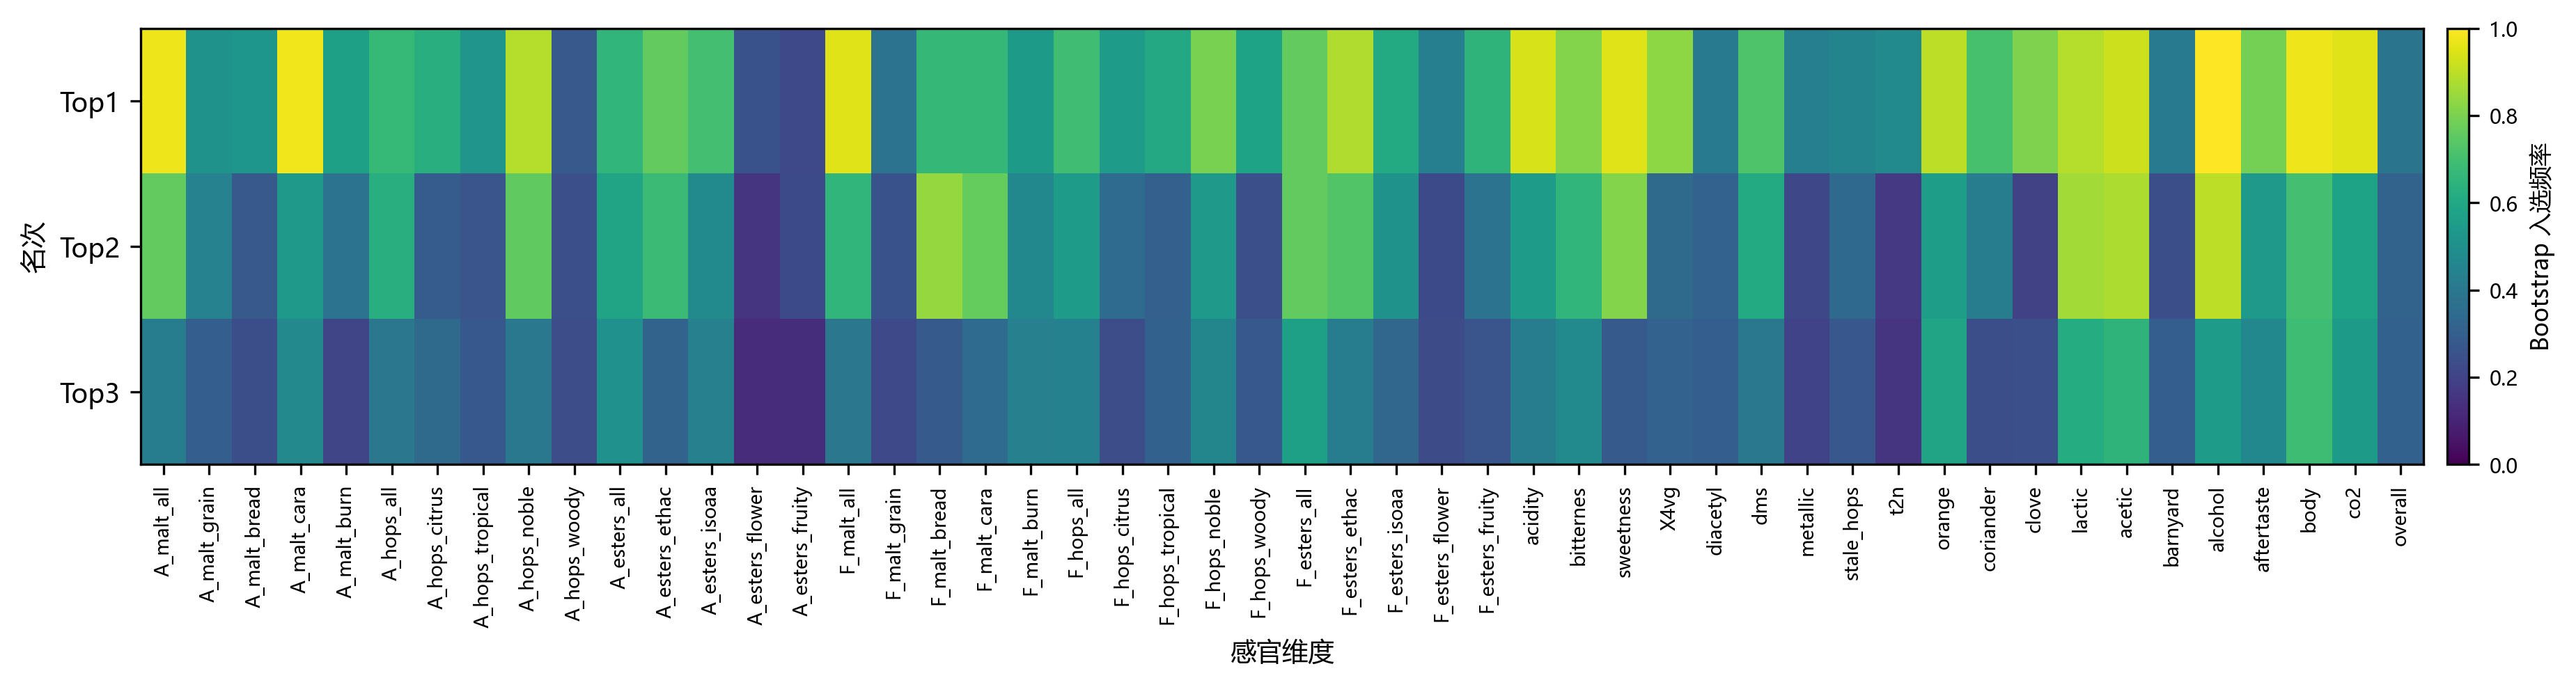
\includegraphics[width=0.98\textwidth]{图M2-02-稳定性频率.png}
\caption{\textbf{50} 个感官维度 Top-3 化合物在 \textbf{200} 次 bootstrap 中的入选频率}
\label{fig:q2-stability}
\end{figure}

图 \ref{fig:q2-stability} 的列是感官维度，行是名次，颜色越亮表示频率越高。亮色主要集中在 Top1 行，Top3 行整体偏暗；这说明“谁是第一”相对稳定，“第三是谁”在很多维度上并不稳定。本文不把这种结果包装成“高度稳定”，也不据此替换 Top-3：频率只用于解释，不用于改排名。若实际应用更看重召回率，可以把 Top-3 当作候选集，再用实验验证后位化合物。

\subsubsection{图项的作用}

$\lambda=0$ 与 $\lambda=0.70$ 的 \textbf{50} 维 Top-3 平均 Jaccard 为 \textbf{0.378}，中位数为 \textbf{0.350}，最小值为 \textbf{0}，最大值为 \textbf{1}。在 \textbf{50} 维中，两种设置重合 \textbf{0} 个、\textbf{1} 个、\textbf{2} 个、\textbf{3} 个的维度分别有 \textbf{3}、\textbf{22}、\textbf{21}、\textbf{4} 个。融合分与直接相关分的跨化合物秩相关均值为 \textbf{0.8693}，最小值为 \textbf{0.8137}；图项得分的跨化合物标准差约为直接相关得分的 \textbf{0.5087} 倍。

\begin{figure}[H]
\centering
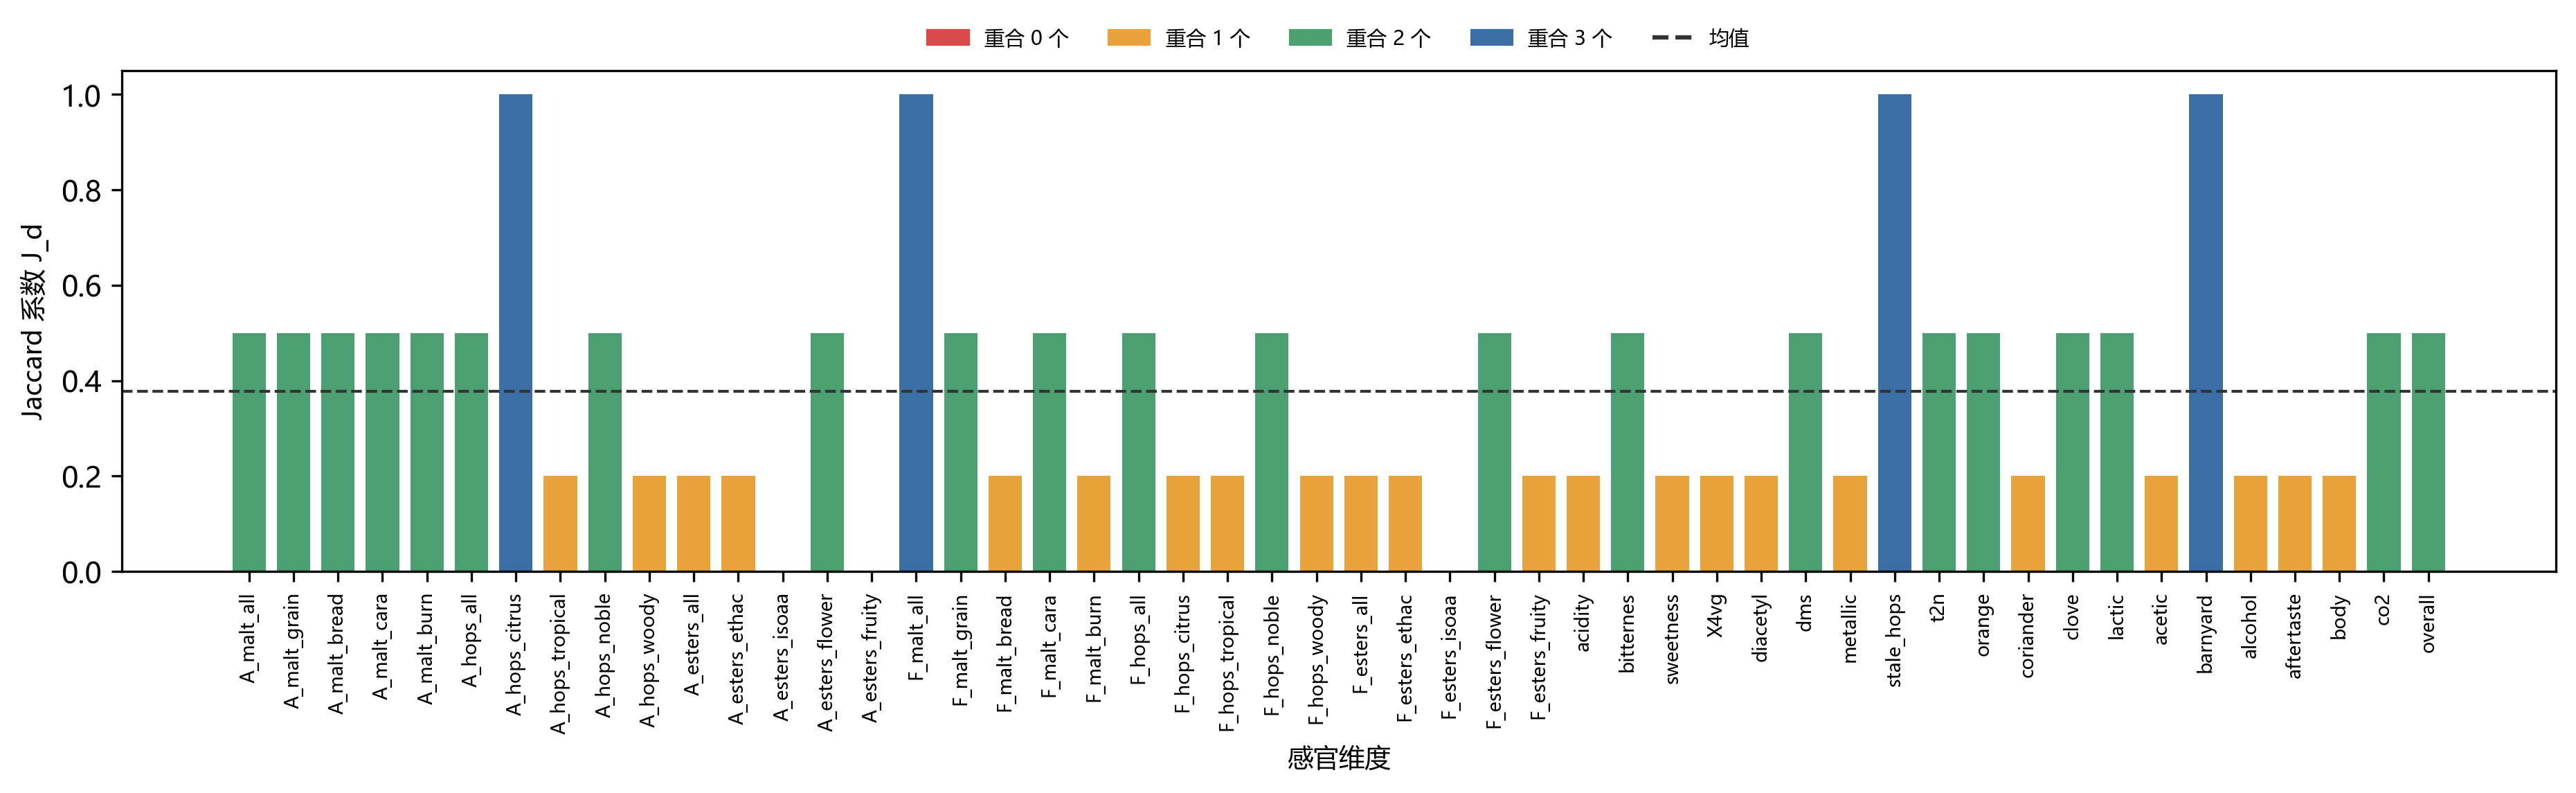
\includegraphics[width=0.98\textwidth]{图M2-03-lambda对照Jaccard.png}
\caption{$\lambda=0$ 与 $\lambda=0.70$ 两种设置下 \textbf{50} 维 Top-3 的逐维 Jaccard 系数}
\label{fig:q2-lambda}
\end{figure}

图 \ref{fig:q2-lambda} 把逐维重合度画成条形图，虚线为 \textbf{50} 维均值 \textbf{0.378}。若图项完全不起作用，所有柱子都应为 \textbf{1}；实际只有 \textbf{4} 维达到 \textbf{1}，多数维度在 \textbf{0.2--0.5} 之间，说明图项确实改变了排序。秩相关 \textbf{0.8693} 又说明融合没有把原排序彻底打乱，图项是在原排序上做局部平滑，而不是另起一套排序。

\subsubsection{化学合理性}

按来源品类核对 \textbf{150} 个 Top-3 格子，一致 \textbf{48} 对、不一致 \textbf{86} 对、不可比 \textbf{16} 对，一致率为 \textbf{0.3582089552}，独立假设基线为 \textbf{0.2047}。不可比的 \textbf{16} 格由两部分组成：\textbf{3} 个缺失品类维度各 \textbf{3} 格，共 \textbf{9} 格；Spices 来源的化合物进入可比维度 \textbf{7} 格。候选池内不可比化合物共 \textbf{24} 个，其中 Spices \textbf{23} 个、Internal standard solution \textbf{1} 个。

这个一致率高于基线，但离半数仍有距离。原因有三：第一，来源品类是粗粒度标签，同一品类下可能包含化学性质差异很大的化合物；第二，Top-3 由相关强度与图平滑决定，不以品类匹配为目标；第三，Spices 与 Internal standard solution 的化合物在感官维度上没有可比的来源品类，只能从分母剔除。若把不可比项强行并入不一致，一致率会被低估；若把它们并入一致，又会高估。本文保留三分类，是为了让分子分母都可复核。

从具体维度看，化学方向是合理的：\texttt{acidity} 的 Acetic acid、\texttt{bitternes} 的 Iso-alpha acids、\texttt{sweetness} 的 Sugars、\texttt{X4vg} 的 4-vinylguaiacol、\texttt{alcohol} 的 Ethanol 都是该感官的已知主要贡献物；\texttt{F\_esters\_ethac} 的 Ethyl propionate 与 Ethyl acetate 属于酯香，\texttt{A\_malt\_all} 的 Color 与 Methylpyrazine 属于麦芽/烘烤方向。与此同时，\texttt{A\_hops\_citrus} 的 Carbon dioxide 与 \texttt{F\_malt\_bread} 的 Betaglucan 更像“相关邻居”而不是直接呈香物，这提示图平滑在带来稳定性的同时，也会引入间接关联。

\subsubsection{GBM 全局对照}

把 \textbf{50} 维 Top-3 合并去重后得到 \textbf{60} 个化合物，它们与 \texttt{8.xlsx} 的 GBM 重要度表交集为 \textbf{60} 个，占选中化合物的 \textbf{100\%}，占 MDI 表的 \textbf{25.974\%}。选中化合物的 MDI 平均分位为 \textbf{0.6201}，\textbf{226} 池的平均分位为 \textbf{0.4971}。

这里必须加一条\textbf{恒真注}：\textbf{60/60} 的重合由“\textbf{226} 候选池是 \textbf{231} 特征子集”这一集合包含关系直接保证，信息量为零，不能把它读成“本文排序与 GBM 重要度一致”。有信息量的是平均分位 \textbf{0.6201} 对 \textbf{0.4971}：它说明本文选中的化合物在 GBM 全局重要度上略高于候选池平均，但差距不大，且 GBM 表没有逐维信息，不能做逐维对照。本文只把它当作全局旁证，不参与 Top-3 的任何计算。

\subsubsection{稳健性检查}

把 $\tau$ 调到 \textbf{0.25} 和 \textbf{0.35}，平均 Jaccard 分别为 \textbf{0.636} 和 \textbf{0.674}；去掉负边只保留正边，平均 Jaccard 为 \textbf{0.648}；把 $\lambda$ 调到 \textbf{0.30} 和 \textbf{0.50}，平均 Jaccard 分别为 \textbf{0.464} 和 \textbf{0.642}。所有扰动下都没有出现“Top-3 完全不变”或“完全改变”的极端，说明主结果对阈值和权重有中等程度的敏感性。

\begin{figure}[H]
\centering
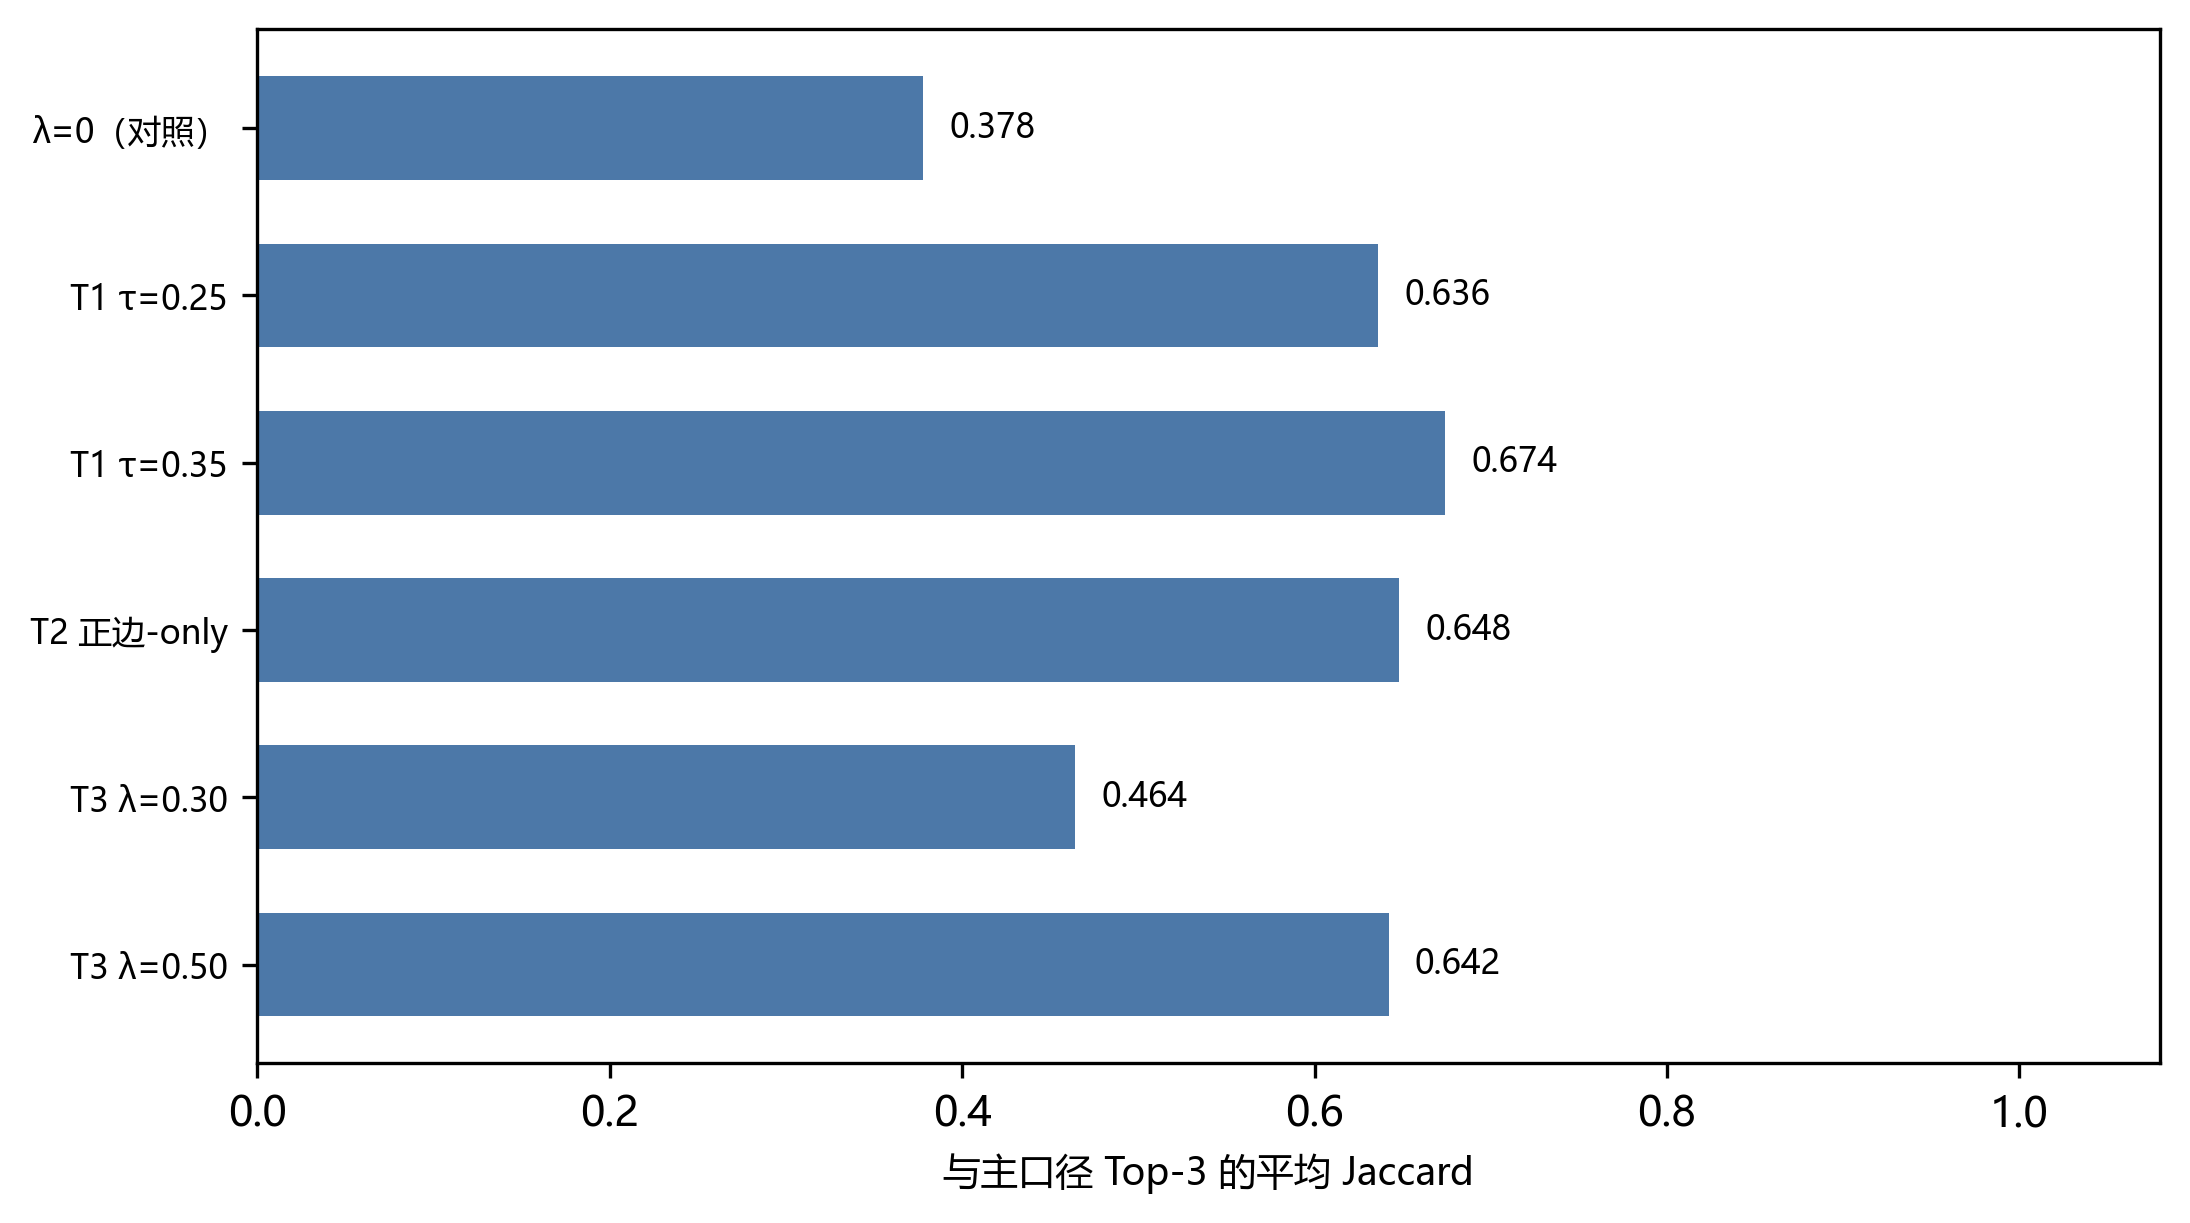
\includegraphics[width=0.82\textwidth]{图M2-04-稳健性检查.png}
\caption{不同图口径与权重设置下 Top-3 与主口径的平均 Jaccard}
\label{fig:q2-robust}
\end{figure}

图 \ref{fig:q2-robust} 中，$\lambda=0.30$ 的 Jaccard 最低（\textbf{0.464}），说明图项权重减半会明显改变后位排序；$\tau=0.35$ 的 Jaccard 最高（\textbf{0.674}），说明把边阈值收紧后，保留的强边足以维持大部分 Top-3。正边-only 的 \textbf{0.648} 说明负边不是排序的主要来源，但去掉负边仍会改变约三分之一的格子，因此负边按绝对值计入是有影响的建模选择，不是可有可无的细节。

\subsubsection{小结}

问题二给出了 \textbf{226} 节点、\textbf{3758} 条边的共表达网络，并用直接相关与图平滑的融合分为每个感官维度选出 Top-3。Top-1 的稳定性高于后两位，图项确实改变了排序，化学方向在多个维度上可解释，但品类一致率只有 \textbf{0.3582}，说明“相关结构上的关键化合物”与“来源品类上的典型化合物”并不是同一个概念。GBM 对照的 \textbf{60/60} 是恒真校验，真正有信息量的是平均分位 \textbf{0.6201} 对 \textbf{0.4971}。这些结果共同支持一个谨慎的结论：本文的 Top-3 可以作为实验验证的候选集，而不宜被当作唯一的因果解释。

\section{问题三：风格条件生成与跨风格迁移}

\noindent\textbf{待 M6 补。}

本章只登记题面要求与拟采用路线，不报告任何生成结果。问题三的实验、图表与数值留待后续里程碑完成。

\subsection{题面要求}

题面要求以啤酒风格为条件，学习一个能够生成化合物谱与对应感官画像的模型，并考察生成结果在不同风格之间的迁移能力。生成结果需要满足三类约束：其一，化合物谱的维度、量纲与训练数据一致，不能生成数据中不存在的化合物；其二，感官画像要与给定风格的目标一致，不能只生成“平均啤酒”；其三，跨风格迁移要能保留源风格的主要特征，同时把目标风格的关键差异迁移过去。

与问题一、问题二相比，这一问的难点从“判别”转为“生成”。判别模型只需要给出一个条件均值或一个排序，生成模型却要刻画整个条件分布；如果只用均方误差训练，生成结果会趋向条件均值，失去样本多样性。另一方面，风格标签的样本量不均衡，少数风格可能只有很少的样本，生成器容易记住多数风格而忽略少数风格。题面还要求化学可解释，这意味着生成器不能只追求与感官标签的拟合，还要满足非负、量纲一致、关键化合物可追溯等约束。

\subsection{拟采用路线}

本文拟采用“风格条件编码—化合物谱生成—感官回评—化学约束”的四段式路线。

第一段是风格条件编码。把风格标签映射为条件向量，条件向量既可以直接用 one-hot 编码，也可以用风格共现结构做嵌入。对样本量较少的风格，嵌入可以共享相似风格的统计强度，避免每个风格单独一套参数。

第二段是化合物谱生成。优先尝试条件变分自编码器：编码器把真实化合物谱压到隐空间，解码器在风格条件与隐变量的共同作用下重建化合物谱；训练目标由重构误差与隐空间正则项组成。若条件变分自编码器的生成样本在化学有效性上不足，再比较条件扩散模型；后者的生成质量通常更好，但采样成本更高，且对超参数更敏感。无论选哪一种，都把问题二得到的关键化合物作为条件中的显式输入，而不是让生成器完全自己发现。

第三段是感官回评。把生成化合物谱送入问题一的随机森林预测器，得到感官画像；再把画像与目标风格的代表性画像比较。回评器在这里只作为“代理评委”，不能替代真实品评；它的作用是快速筛掉明显偏离目标风格的生成样本，并为生成器提供可微或可采样的反馈信号。

第四段是化学约束。对生成化合物谱施加非负约束、量纲约束与聚合量一致性约束；对题面点名的缺陷化合物，按已登记的阈值表检查是否超阈值；对无法从数据确认的约束，明确写成“资料未覆盖”，不用猜测补位。

\subsection{跨风格迁移与验证设计}

跨风格迁移拟采用“源风格编码 + 目标风格条件”的方式：固定源风格的隐变量或内容变量，替换目标风格的条件向量，观察生成化合物谱与感官画像的变化。为了避免把“换了一个随机种子”误读为迁移，验证时固定随机源，并对同一源样本做多次条件替换，比较迁移前后关键化合物的变化方向。

验证设计分四层。第一层是化学有效性：生成谱是否非负、量纲是否与训练数据一致、聚合量是否与分项大致协调。第二层是感官一致性：回评画像与目标风格的代表性画像在主要感官维度上是否同向。第三层是多样性：同一风格条件下生成的不同样本不能完全相同，否则说明模型只记住了条件均值。第四层是迁移性：源风格的主要特征在迁移后是否保留，目标风格的关键差异是否出现。四层都只写验证方案，具体指标与结果留待后续里程碑。

\subsection{风险与边界}

主要风险有三类。第一，风格样本不均衡导致少数风格生成质量差；应对方式是把风格分层纳入采样与评估，而不是只看总体平均。第二，生成器只拟合感官标签、忽略化学约束，产生“感官像、化学不像”的样本；应对方式是把化学约束放在生成之后、回评之前，先过滤再评价。第三，回评器本身有误差，生成器可能利用回评器的弱维“钻空子”；应对方式是对回评器的不确定维度降权，并用独立证据做交叉核对。

本章不给出任何生成结果、图表或数值。问题三的模型选择、参数、生成样本与跨风格迁移实验，均在第 M6 阶段完成并并入论文。

\section{模型评价、结论与建议}

\subsection{模型评价}

本文模型的优点主要有四点。第一，问题一把随机森林与 ALR 标定拆成“连续拟合”和“等级映射”两层，前者负责非线性与交互，后者负责题面要求的整数刻度，两层各自可检验，出了问题能定位到具体一层。第二，模型选择采用两阶段预注册，阈值、折索引、特征集都在结果产生之前冻结，避免了“看测试集挑模型”的选择偏差。第三，问题二把直接相关与图平滑写成可加融合分，并用 bootstrap、阈值扰动、负边消融与权重扰动四种方式检查，结论不依赖单一设置。第四，本文没有把 T2、T7、T8 的偏离包装成“模型很好”，而是给出刻度不可达命题与可读口径辅助表，既保留主表的契约口径，又让读者能按题面等级阅读。

模型的不足也有三点。第一，平均 $R^2$ 只有 \textbf{0.2305}（折均）与 \textbf{0.2565}（OOF 全局），部分弱维的逐维 $R^2$ 接近零甚至为负，说明化合物信息不足以解释所有感官差异。第二，问题二的 Top-1 较稳，但 Top-3 后两位的 bootstrap 频率偏低，第三名平均只有 \textbf{0.3611}，实际使用时不宜把 Top-3 当作同等可靠的结论。第三，问题三尚未开展实验，风格条件生成与跨风格迁移只有路线，没有结果；这是本阶段的边界，不是可以含糊带过的部分。

\subsection{结论}

\textbf{问题一}：随机森林与 \textbf{226} 维 F0 特征集是当前数据下的合理选择，OOF 全局 $R^2$ 为 \textbf{0.2565}，折均 $R^2$ 为 \textbf{0.2305}，均高于同口径基线。ALR 把连续预测转成 \textbf{0--6} 级；主表 \textbf{0} 级与 \textbf{6} 级为空是刻度不可达命题的必然结果，不是实现缺陷。可读口径辅助表在保持同序（逆序对 \textbf{0}）的前提下让 \textbf{7} 级全部出现，解决了“看起来没有 \textbf{6} 级”的阅读问题。

\textbf{问题二}：\textbf{226} 个候选化合物、\textbf{3758} 条边构成共表达网络，融合分在 $\lambda=0.70$ 下给出每个感官维度的 Top-3。Top-1 的平均入选频率为 \textbf{0.6734}，Top-3 为 \textbf{0.3611}；图项使 Top-3 相对直接相关的平均 Jaccard 降到 \textbf{0.378}，说明图结构确实参与排序。品类一致率为 \textbf{0.3582}，高于独立基线 \textbf{0.2047}，但离半数仍有距离；GBM 的 \textbf{60/60} 重合是恒真校验，有信息量的是平均分位 \textbf{0.6201} 对 \textbf{0.4971}。这些结果支持把 Top-3 作为实验候选集，而不是唯一因果解释。

\textbf{问题三}：待 M6 补。

\subsection{建议}

对酿造实践，本文给出三条建议。第一，优先用各维度的 Top-1 做靶向实验，把 Top-2 与 Top-3 作为备选；Top-1 的 bootstrap 频率明显高于后两位，直接拿第三名做工艺调整的风险较大。第二，使用评分表时同时保留主表与可读口径表：主表用于与训练标签同刻度的契约口径，可读表用于按题面等级展示；两者单调同序，不能互相替代，也不应把可读表当成新的训练目标。第三，后续数据采集应优先补强弱维与少数风格：弱维的逐维 $R^2$ 低，说明现有化合物面板缺少能解释这些感官的信息；少数风格样本少，会直接影响问题三的条件生成与迁移评估。

对后续建模，本文建议在问题三中把“化学有效性”放在“感官拟合”之前：先保证生成谱非负、量纲一致、关键化合物可追溯，再谈感官画像是否像目标风格。回评器可以使用问题一的随机森林，但必须对弱维降权，并用独立证据交叉核对，避免生成器利用回评器的误差“钻空子”。

\section{参考文献}

\begingroup
\renewcommand{\refname}{}
\bibliographystyle{gbt7714-numerical}
\bibliography{refs}
\endgroup

\section{附录}

\subsection{AI 使用声明}

本论文在数据核验、编程实现、图表生成与文字起草环节使用了人工智能工具辅助。工具名称：DeepSeek Harness；版本/型号：deepseek-flash；开发机构/公司：深度求索（DeepSeek）；版本发布日期：2026-10-24（本次运行所用版本）。

具体使用环节如下：其一，数据口径核对与结果文件整理，由 AI 辅助读取与比对，最终数值以编程角色的结果文件为准；其二，问题一、问题二的建模代码与图表由 AI 辅助编写和生成，代码文件头已按要求写明 AI 工具、版本、机构与日期；其三，论文初稿的结构、段落与表格由 AI 辅助起草，队员对模型设定、数值与结论逐条复核；其四，文献线索与格式由 AI 辅助整理，引用条目均给出 DOI 或 URL，正文引用与文献表一一对应。

逐处标注体例采用“来源表 + 题注 + 附录声明”三级。第一级是数值：正文中出现的每个定量结果都登记在数字源对照表中，给出源文件与列/行，正文不写无源数字。第二级是图表：每张图的题注注明图集稳定编号与数据来源，每个表的表注注明结果文件；图内不烧编号，编号由 LaTeX 自动生成。第三级是文字：AI 参与起草的段落统一在本小节声明，正文不把 AI 生成内容写成人工原创；涉及模型设定、公式与结论的句子由队员改写或复核。本文未使用无法溯源的模型或公式；所有公式均有文献依据或由本文给出推导。

本队对论文的全部内容负责。AI 工具只作为辅助手段，不替代本队对数据、模型、结果与结论的判断。

\subsection{复现材料与源码说明}

论文的 LaTeX 主文件为 \texttt{论文/产出/}\allowbreak\texttt{main.tex}，分章源文件位于 \texttt{论文/产出/}\allowbreak\texttt{sections/}，图片位于 \texttt{论文/产出/}\allowbreak\texttt{figs/}，参考文献为 \texttt{论文/产出/}\allowbreak\texttt{refs.bib}。图表与图集的对应关系登记在 \texttt{论文/产出/}\allowbreak\texttt{图表映射.md}，正文数字与结果文件的对应关系登记在 \texttt{论文/产出/}\allowbreak\texttt{数字源对照-M4.csv}。

编译在 \texttt{论文/产出} 目录下执行，顺序为：先运行 \texttt{xelatex main.tex}，再运行 \texttt{bibtex main}，最后再运行两次 \texttt{xelatex main.tex}。四次编译的退出码、日志中的缺字计数与引用计数记录在 \texttt{论文/产出/}\allowbreak\texttt{自检-M4.md}。

问题一的结果文件包括 \texttt{编程/产出/Q1\_核验指标.csv}、\texttt{Q1\_逐维指标.csv}、\texttt{Q1\_分级频数.csv}、\texttt{Q1\_可读口径参数.json} 等；问题二的结果文件包括 \texttt{编程/产出/Q2\_核验指标.csv}、\texttt{Q2\_top3.csv}、\texttt{Q2\_稳健性.csv} 等。论文只读取这些文件，不修改其结果。问题三尚未开展实验，相关章节只登记路线，不包含结果数值。

\begin{table}[H]
\centering
\zihao{-5}
\begin{tabularx}{\textwidth}{@{}p{0.33\textwidth}p{0.47\textwidth}X@{}}
\toprule
文件或目录 & 作用 & 写者 \\
\midrule
\texttt{论文/产出/main.tex} & LaTeX 主文件与编译入口 & 论文 \\
\texttt{论文/产出/sections/} & 九节分章源文件 & 论文 \\
\texttt{论文/产出/figs/} & 从图集复制入文的图片 & 论文 \\
\texttt{论文/产出/refs.bib} & 参考文献条目 & 论文 \\
\texttt{论文/产出/数字源对照-M4.csv} & 正文数字到结果文件的回源表 & 论文 \\
\texttt{论文/产出/图表映射.md} & 论文编号到图集编号的映射 & 论文 \\
\texttt{编程/产出/Q1\_*.csv} & 问题一结果与检验数据 & 编程 \\
\texttt{编程/产出/Q2\_*.csv} & 问题二结果与检验数据 & 编程 \\
\texttt{图集/M2/}、\texttt{图集/M3/} & 论文所用图片的原始文件 & 编程 \\
\bottomrule
\end{tabularx}
\caption{论文复现材料与源码清单}
\label{tab:repro}
\end{table}

\subsection{数据与代码边界}

本文使用的原始数据位于 \texttt{数据/A/}，为只读材料；口径规范、维度映射与阈值表由建模角色产出；结果文件与图集由编程角色产出。论文角色不写生产代码、不改结果文件与图集，只负责组织、解释与排版。若读者发现正文数字与结果文件不一致，应以结果文件为准，并按数字源对照表回溯到具体列/行。

\subsection{提交前复核说明}

提交前在仓库根目录执行 \texttt{python 工具/check\_paths.py}，并在仓库外干净检出中复跑同一脚本与完整编译链；两次输出、缺字计数与页数均记录在自检文件。源文件统一为 UTF-8 无 BOM、LF 换行；图表题注均位于对象下方，图内不写编号。

复现时注意三点。第一，编译顺序必须是 \texttt{xelatex}、\texttt{bibtex}、\texttt{xelatex}、\texttt{xelatex}，只跑两遍 \texttt{xelatex} 会留下未定义引用。第二，中文渲染以日志中的缺字计数和 PDF 目检双重确认，不能只看编译是否退出成功。第三，正文所有定量表述都可在数字源对照表中找到源文件与列/行；若结果文件更新，应先更新对照表，再改正文。


\end{document}
